\documentclass[
	% -- opções da classe memoir --
	12pt,				% tamanho da fonte
	% openright,			% capítulos começam em pág ímpar (insere página vazia caso preciso)
	oneside,			% para impressão apenas no anverso (apenas frente). Oposto a twoside
	a4paper,			% tamanho do papel. 
	% -- opções da classe abntex2 --
	%chapter=TITLE,		% títulos de capítulos convertidos em letras maiúsculas
	%section=TITLE,		% títulos de seções convertidos em letras maiúsculas
	%subsection=TITLE,	% títulos de subseções convertidos em letras maiúsculas
	%subsubsection=TITLE,% títulos de subsubseções convertidos em letras maiúsculas
	% -- opções do pacote babel --
	english,			% idioma adicional para hifenização
	%french,				% idioma adicional para hifenização
	%spanish,			% idioma adicional para hifenização
	brazil				% o último idioma é o principal do documento
	]{abntex2ppgsi}

% ---
% Pacotes básicos 
% ---
% \usepackage{lmodern}			% Usa a fonte Latin Modern			
% \usepackage[T1]{fontenc}		% Selecao de codigos de fonte.
\usepackage[utf8]{inputenc}		% Codificacao do documento (conversão automática dos acentos)
\usepackage{lastpage}			% Usado pela Ficha catalográfica
\usepackage{indentfirst}		% Indenta o primeiro parágrafo de cada seção.
\usepackage{color}				% Controle das cores
\usepackage{colortbl}
\usepackage{graphicx}			% Inclusão de gráficos
\usepackage{subcaption}			% Inclusão de subfiguras
\usepackage{microtype} 			% para melhorias de justificação
\usepackage{pdfpages}     %para incluir pdf
\usepackage{algorithm}			%para ilustrações do tipo algoritmo
\usepackage{mdwlist}			%para itens com espaço padrão da abnt
\usepackage[noend]{algpseudocode}			%para ilustrações do tipo algoritmo
\usepackage{longtable}
\usepackage{multirow}
\usepackage{lscape}
\usepackage{listings}
\definecolor{verde}{rgb}{0.25,0.5,0.35}
\definecolor{jpurple}{rgb}{0.5,0,0.35}
\usepackage{xcolor}
\usepackage{multirow}

\lstset{
	language=Java,
	basicstyle=\ttfamily\small,
	keywordstyle=\color{jpurple}\bfseries,
	stringstyle=\color{red},
	commentstyle=\color{verde},
	morecomment=[s][\color{blue}]{/**}{*/},
	extendedchars=true,
	showspaces=false,
	showstringspaces=false,
	numbers=left,
	numberstyle=\tiny,
	breaklines=true,
	backgroundcolor=\color{cyan!10},
	breakautoindent=true,
	captionpos=b,
	xleftmargin=0pt,
	tabsize=4
}

\lstset{
	language=Python,
	basicstyle=\ttfamily\small,
	keywordstyle=\color{jpurple}\bfseries,
	stringstyle=\color{red},
	commentstyle=\color{verde},
	morecomment=[s][\color{blue}]{/**}{*/},
	extendedchars=true,
	showspaces=false,
	showstringspaces=false,
	numbers=left,
	numberstyle=\tiny,
	breaklines=true,
	backgroundcolor=\color{cyan!10},
	breakautoindent=true,
	captionpos=b,
	xleftmargin=0pt,
	tabsize=4
}
		
% ---
% Pacotes adicionais, usados apenas no âmbito do Modelo Canônico do abnteX2
% ---
\usepackage{lipsum}				% para geração de dummy text
% ---

% ---
% Pacotes de citações
% ---
\usepackage[brazilian,hyperpageref]{backref}	 % Paginas com as citações na bibl
\usepackage[alf]{abntex2cite}	% Citações padrão ABNT

% --- 
% CONFIGURAÇÕES DE PACOTES
% --- 

% ---
% Configurações do pacote backref
% Usado sem a opção hyperpageref de backref
\renewcommand{\backrefpagesname}{Citado na(s) página(s):~}
% Texto padrão antes do número das páginas
\renewcommand{\backref}{}
% Define os textos da citação
\renewcommand*{\backrefalt}[4]{
	\ifcase #1 %
		Nenhuma citação no texto.%
	\or
		Citado na página #2.%
	\else
		Citado #1 vezes nas páginas #2.%
	\fi}%
% ---

% ---
% Informações de dados para CAPA e FOLHA DE ROSTO
% ---

%-------------------------------------------------------------------------
% Comentário adicional do PPgSI - Informações sobre o ``título'':
%
% Em maiúscula apenas a primeira letra da sentença (do título), exceto 
% nomes próprios, geográficos, institucionais ou Programas ou Projetos ou 
% siglas, os quais podem ter letras em maiúscula também.
%
% O subtítulo do trabalho é opcional.
% Sem ponto final.
%
% Atenção: o título da Dissertação na versão corrigida não pode mudar. 
% Ele deve ser idêntico ao da versão original.
%
%-------------------------------------------------------------------------
\titulo{I9Vanets: um modelo de arquitetura de software para rede veicular}

%-------------------------------------------------------------------------
% Comentário adicional do PPgSI - Informações sobre o ``autor'':
%
% Todas as letras em maiúsculas.
% Nome completo.
% Sem ponto final.
%-------------------------------------------------------------------------
\autor{\uppercase{George Leite Junior}}

%-------------------------------------------------------------------------
% Comentário adicional do PPgSI - Informações sobre o ``local'':
%
% Não incluir o ``estado''.
% Sem ponto final.
%-------------------------------------------------------------------------
\local{São Cristóvão}

%-------------------------------------------------------------------------
% Comentário adicional do PPgSI - Informações sobre a ``data'':
%
% Colocar o ano do depósito (ou seja, o ano da entrega) da respectiva 
% versão, seja ela a versão original (para a defesa) seja ela a versão 
% corrigida (depois da aprovação na defesa). 
%
% Atenção: Se a versão original for depositada no final do ano e a versão 
% corrigida for entregue no ano seguinte, o ano precisa ser atualizado no 
% caso da versão corrigida. 
% Cuidado, pois o ano da ``capa externa'' também precisa ser atualizado 
% nesse caso.
%
% Não incluir o dia, nem o mês.
% Sem ponto final.
%-------------------------------------------------------------------------
\data{2016}

%-------------------------------------------------------------------------
% Comentário adicional do PPgSI - Informações sobre o ``Orientador'':
%
% Se for uma professora, trocar por ``Profa. Dra.''
% Nome completo.
% Sem ponto final.
%-------------------------------------------------------------------------
\orientador{Prof.ª Dr.ª Douglas D. J. de Macedo}

%-------------------------------------------------------------------------
% Comentário adicional do PPgSI - Informações sobre o ``Coorientador'':
%
% Opcional. Incluir apenas se houver co-orientador formal, de acordo com o 
% Regulamento do Programa.
%
% Se for uma professora, trocar por ``Profa. Dra.''
% Nome completo.
% Sem ponto final.
%-------------------------------------------------------------------------
\coorientador{Prof. Dr. Rogério Patrício Chagas do Nascimento }

\tipotrabalho{Dissertação (Mestrado)}

\preambulo{
%-------------------------------------------------------------------------
% Comentário adicional do PPgSI - Informações sobre o texto ``Versão 
% original'':
%
% Não usar para Qualificação.
% Não usar para versão corrigida de Dissertação.
%
%-------------------------------------------------------------------------
Versão original
%-------------------------------------------------------------------------
% Comentário adicional do PPgSI - Informações sobre o ``texto principal do
% preambulo'':
%
% Para Qualificação, trocar por: Texto de Exame de Qualificação apresentado à Escola de Artes, Ciências e Humanidades da Universidade de São Paulo como parte dos requisitos para obtenção do título de Mestre em Ciências pelo Programa de Pós-graduação em Sistemas de Informação.
%
%-------------------------------------------------------------------------
\newline \newline \newline Dissertação apresentada à Pró-Reitoria de Pós-Graduação e Pesquisa da Universidade Federal de Sergipe para obtenção do título de Mestre em Ciência da Computação pelo Programa de Pós-graduação em Ciência da Computação.
%
\newline \newline Área de concentração: Redes de Computadores e Sistemas Distribuídos
%-------------------------------------------------------------------------
% Comentário adicional do PPgSI - Informações sobre o texto da ``Versão 
% corrigida'':
%
% Não usar para Qualificação.
% Não usar para versão original de Dissertação.
% 
% Substituir ``xx de xxxxxxxxxxxxxxx de xxxx'' pela ``data da defesa''.
%
%-------------------------------------------------------------------------
%\newline \newline \newline Versão corrigida contendo as alterações solicitadas pela comissão %julgadora em xx de xxxxxxxxxxxxxxx de xxxx. A versão original encontra-se em acervo reservado %na Biblioteca da EACH-USP e na Biblioteca Digital de Teses e Dissertações da USP (BDTD), de %acordo com a Resolução CoPGr 6018, de 13 de outubro de 2011.
}
% ---


% ---
% Configurações de aparência do PDF final

% alterando o aspecto da cor azul
\definecolor{blue}{RGB}{41,5,195}
\definecolor{red}{RGB}{255,0,0}
\definecolor{yellow}{RGB}{255,241,0}
\definecolor{green}{RGB}{0,255,0}
\definecolor{orange}{RGB}{255,153,51}
\definecolor{gray}{RGB}{127,127,127}



% informações do PDF
\makeatletter
\hypersetup{
     	%pagebackref=true,
		pdftitle={\@title}, 
		pdfauthor={\@author},
    	pdfsubject={\imprimirpreambulo},
	    pdfcreator={LaTeX com abnTeX2 adaptado para o PPgSI-EACH-USP},
		pdfkeywords={abnt}{latex}{abntex}{abntex2}{qualificação de mestrado}{dissertação de mestrado}{ppgsi}, 
		colorlinks=true,       		% false: boxed links; true: colored links
    	linkcolor=blue,          	% color of internal links
    	citecolor=blue,        		% color of links to bibliography
    	filecolor=magenta,      		% color of file links
		urlcolor=blue,
		bookmarksdepth=4
}
\makeatother
% --- 

% --- 
% Espaçamentos entre linhas e parágrafos 
% --- 

% O tamanho do parágrafo é dado por:
\setlength{\parindent}{1.25cm}

% Controle do espaçamento entre um parágrafo e outro:
\setlength{\parskip}{0cm}  % tente também \onelineskip
\renewcommand{\baselinestretch}{1.5}

% ---
% compila o indice
% ---
\makeindex
% ---

	% Controlar linhas orfas e viuvas
  \clubpenalty10000
  \widowpenalty10000
  \displaywidowpenalty10000

% ----
% Início do documento
% ----
\begin{document}

% Retira espaço extra obsoleto entre as frases.
\frenchspacing 

% ----------------------------------------------------------
% ELEMENTOS PRÉ-TEXTUAIS
% ----------------------------------------------------------
% \pretextual

% ---
% Capa
% ---
%-------------------------------------------------------------------------
% Comentário adicional do PPgSI - Informações sobre a ``capa'':
%
% Esta é a ``capa'' principal/oficial do trabalho, a ser impressa apenas 
% para os casos de encadernação simples (ou seja, em ``espiral'' com 
% plástico na frente).
% 
% Não imprimir esta ``capa'' quando houver ``capa dura'' ou ``capa brochura'' 
% em que estas mesmas informações já estão presentes nela.
%
%-------------------------------------------------------------------------
\imprimircapa
% ---

% ---
% Folha de rosto
% (o * indica que haverá a ficha bibliográfica)
% ---
\imprimirfolhaderosto*
% ---

% ---
% Inserir a autorização para reprodução e ficha bibliografica
% ---

%-------------------------------------------------------------------------
% Comentário adicional do PPgSI - Informações sobre o texto da 
% ``autorização para reprodução e ficha bibliografica'':
%
% Página a ser usada apenas para Dissertação (tanto na versão original 
% quanto na versão corrigida).
%
% Solicitar a ficha catalográfica na Biblioteca da EACH. 
% Duas versões devem ser solicitadas, em dois momentos distintos: uma vez 
% para a versão original, e depois outra atualizada para a versão 
% corrigida.
%
% Atenção: esta página de ``autorização para reprodução e ficha 
% catalográfica'' deve ser impressa obrigatoriamente no verso da folha de 
% rosto.
%
% Não usar esta página para Qualificação.
%
% Substitua o arquivo ``fig_ficha_catalografica.pdf'' abaixo referenciado 
% pelo PDF elaborado pela Biblioteca
%
%-------------------------------------------------------------------------
%\begin{fichacatalografica}
%    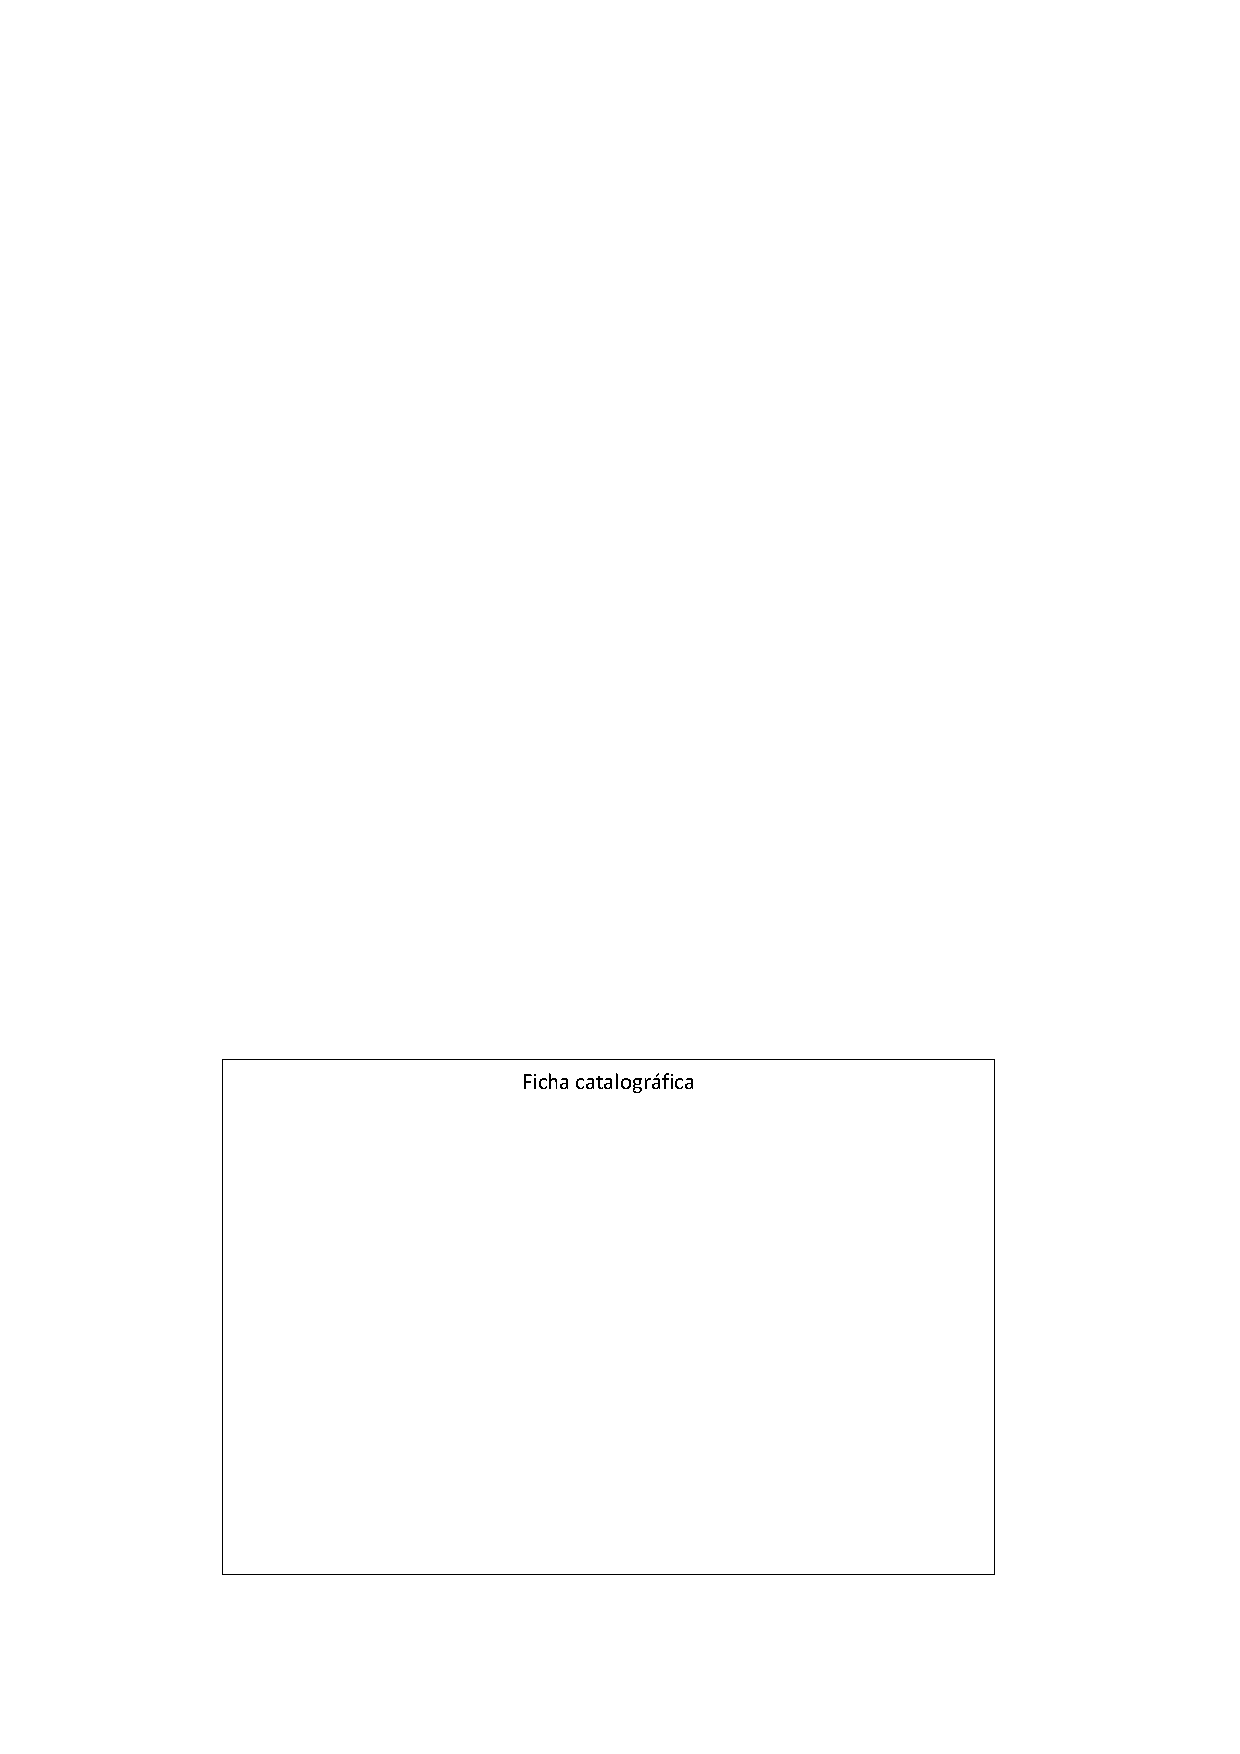
\includepdf{fig_ficha_catalografica.pdf}
%\end{fichacatalografica}

% ---
% Inserir errata
% ---
%-------------------------------------------------------------------------
% Comentário adicional do PPgSI - Informações sobre ``Errata'':
%
% Usar esta página de errata apenas em casos de excepcionais, e apenas 
% para a versão corrigida da Dissertação. Por exemplo, quando depois de
% já depositada e publicada a versão corrigida, ainda assim verifica-se
% a necessidade de alguma correção adicional.
%
% Se precisar usar esta página, busque a forma correta (o modelo correto) 
% para fazê-lo, de acordo com a norma ABNT.
%
% Não usar esta página para versão original de Dissertação.
% Não usar esta página para Qualificação.
%
%-------------------------------------------------------------------------
%\begin{errata}
%Elemento opcional para versão corrigida, depois de depositada.
%\end{errata}
% ---

% ---
% Inserir folha de aprovação
% ---

\begin{folhadeaprovacao}
%-------------------------------------------------------------------------
% Comentário adicional do PPgSI - Informações sobre ``Folha da aprovação'':
%
% Para Qualificação, trocar por: Texto de Exame de Qualificação de autoria de Fulano de Tal, sob o título \textbf{``\imprimirtitulo''}, apresentado à Escola de Artes, Ciências e Humanidades da Universidade de São Paulo, como parte dos requisitos para obtenção do título de Mestre em Ciências pelo Programa de Pós-graduação em Sistemas de Informação, na área de concentração Metodologia e Técnicas da Computação, aprovado em \_\_\_ de \_\_\_\_\_\_\_\_\_\_\_\_\_\_ de \_\_\_\_\_\_ pela comissão examinadora constituída pelos doutores:
%
% Substituir ``Fulano de Tal'' pelo nome completo do autor do trabalho, com 
% apenas as iniciais em maiúsculo.
%
% Substiuir ``___ de ______________ de ______'' por: 
%     - Para versão original de Dissertação: deixar em branco, pois a data 
%       pode mudar, mesmo que ela já esteja prevista.
%     - Para versão corrigida de Dissertação: usar a data em que a defesa 
%       efetivamente ocorreu.
%
%-------------------------------------------------------------------------
\noindent Dissertação de autoria de George Leite Junior, sob o título \textbf{``\imprimirtitulo''}, apresentada à Pró-Reitoria de Pós-Graduação e Pesquisa da Universidade Federal de Sergipe, para obtenção do título de Mestre em Ciência da Computação pelo Programa de Pós-graduação em Ciência da Computação, na área de concentração Redes de Computadores e Sistemas Distribuídos, aprovada em \_\_\_\_\_ de \_\_\_\_\_\_\_\_\_\_\_\_\_\_\_\_\_\_ de \_\_\_\_\_\_\_\_ pela comissão julgadora constituída pelos doutores:

\vspace*{3cm}

\begin{center}
%-------------------------------------------------------------------------
% Comentário adicional do PPgSI - Informações sobre ``assinaturas'':
%
% Para Qualificação e para versão original de Dissertação: deixar em 
% branco (ou seja, assim como está abaixo), pois os membros da banca podem
% mudar, mesmo que eles já estejam previstos.
% 
% Para versão corrigida de Dissertação: usar os dados dos examinadores que 
% efetivamente participaram da defesa. 
% 
% Em nenhum caso há realmente necessidade de assinaturas.
%
% Para versão corrigida de Dissertação: em caso de ``professora'', trocar 
% por ``Profa. Dra.'' 
% 
% Para versão corrigida de Dissertação: ao colocar os nomes dos 
% examinadores, remover o sublinhado
% 
% Para versão corrigida de Dissertação: ao colocar os nomes dos 
% examinadores, usar seus nomes completos, exatamente conforme constam em 
% seus Currículos Lattes
% 
% Para versão corrigida de Dissertação: ao colocar os nomes das 
% instituições, remover o sublinhado e remover a palavra ``Instituição:''
%
% Não abreviar os nomes das instituições.
%
%-------------------------------------------------------------------------
\textbf{Prof.ª Dr.ª \_\_\_\_\_\_\_\_\_\_\_\_\_\_\_\_\_\_\_\_\_\_\_\_\_\_\_\_\_\_\_\_\_\_\_\_\_\_\_\_\_\_} 
\\ Presidente 
\\ Instituição: \_\_\_\_\_\_\_\_\_\_\_\_\_\_\_\_\_\_\_\_\_\_\_\_\_\_\_\_\_\_\_\_\_\_\_\_\_\_\_\_\_\_ 

\vspace*{2cm}

\textbf{Prof. Dr. \_\_\_\_\_\_\_\_\_\_\_\_\_\_\_\_\_\_\_\_\_\_\_\_\_\_\_\_\_\_\_\_\_\_\_\_\_\_\_} 
\\ Instituição: \_\_\_\_\_\_\_\_\_\_\_\_\_\_\_\_\_\_\_\_\_\_\_\_\_\_\_\_\_\_\_\_\_\_\_\_\_\_\_\_

\vspace*{2cm}

\textbf{Prof. Dr. \_\_\_\_\_\_\_\_\_\_\_\_\_\_\_\_\_\_\_\_\_\_\_\_\_\_\_\_\_\_\_\_\_\_\_\_\_\_\_} 
\\ Instituição: \_\_\_\_\_\_\_\_\_\_\_\_\_\_\_\_\_\_\_\_\_\_\_\_\_\_\_\_\_\_\_\_\_\_\_\_\_\_\_\_

\end{center}
  
\end{folhadeaprovacao}
% ---

% ---
% Dedicatória
% ---
%-------------------------------------------------------------------------
% Comentário adicional do PPgSI - Informações sobre ``Dedicatória'': 
%
% Opcional para Dissertação.
% Não sugerido para Qualificação.
% 
%-------------------------------------------------------------------------
%\begin{dedicatoria}
%   \vspace*{\fill}
%   \centering
%   \noindent
%   \textit{Escreva aqui sua dedicatória, se desejar, ou remova esta página...} 
%	 \vspace*{\fill}
%\end{dedicatoria}
% ---

% ---
% Agradecimentos
% ---
%-------------------------------------------------------------------------
% Comentário adicional do PPgSI - Informações sobre ``Agradecimentos'': 
%
% Opcional para Dissertação.
% Não sugerido para Qualificação.
% 
% Lembrar de agradecer agências de fomento e outras instituições similares.
%
%-------------------------------------------------------------------------
%\begin{agradecimentos}
%Colocar os agradecimentos
%\end{agradecimentos}
% ---

% ---
% Epígrafe
% ---
%-------------------------------------------------------------------------
% Comentário adicional do PPgSI - Informações sobre ``Epígrafe'': 
%
% Opcional para Dissertação.
% Não sugerido para Qualificação.
% 
%-------------------------------------------------------------------------
%\begin{epigrafe}
%    \vspace*{\fill}
%	\begin{flushright}
%		\textit{``Escreva aqui uma epígrafe, se desejar, ou remova esta página...''\\
%		(Autor da epígrafe)}
%	\end{flushright}
%\end{epigrafe}
% ---

% ---
% RESUMOS
% ---

% resumo em português
\setlength{\absparsep}{18pt} % ajusta o espaçamento dos parágrafos do resumo
\begin{resumo}

%-------------------------------------------------------------------------
% Comentário adicional do PPgSI - Informações sobre ``referência'':
% 
% Troque os seguintes campos pelos dados de sua Dissertação (mantendo a 
% formatação e pontuação):
%   - SOBRENOME
%   - Nome1
%   - Nome2
%   - Nome3
%   - Título do trabalho: subtítulo do trabalho
%   - AnoDeDefesa
%
% Mantenha todas as demais informações exatamente como estão.
% 
% [Não usar essas informações de ``referência'' para Qualificação]
%
%----------------------	---------------------------------------------------
\begin{flushleft}
LEITE, George Junior. \textbf{\imprimirtitulo}. \imprimirdata. \pageref{LastPage} f. Dissertação (Mestrado em Ciência da Computação) – Pró-Reitoria de Pós-Graduação e Pesquisa, Universidade Federal de Sergipe, Sergipe, 2016.
\end{flushleft}

Em consequência do crescimento populacional, as grandes cidades enfrentam problemas cotidianos relacionados à mobilidade urbana tais como: congestionamentos, baixa qualidade das rodovias, ineficiência de transportes públicos, entre outros. Iniciativas de sistemas de transportes inteligentes (STI) agem como uma solução eficiente para melhorar o funcionamento e desempenho dos sistemas de tráfego, reduzindo congestionamentos e aumentando a segurança para os cidadãos. Atualmente, pesquisadores vem buscando nas redes veiculares ad-hoc (VANET) uma possível solução para os problemas referentes à mobilidade urbana. Contudo, VANETs ainda apresenta uma série de desafios que devem ser resolvidos para que seu uso seja consolidado.  Deste modo, o presente trabalho apresenta uma arquitetura denominada i9Vanets, cujo intuito é o gerenciamento virtualizado por meio de uma rede veicular para auxiliar nas soluções dos principais desafios relacionados à VANETs. Também é apresentado uma análise, dos testes realizados em laboratório, com objetivo de avaliar seu desempenho e capacidade operacional. Sendo assim, a conclusão deste trabalho, foi apresentar a viabilidade técnica da arquitetura i9Vanets bem como suas possíveis aplicações.


Palavras-chaves: Rede Veicular. Computação em Nuvem.
\end{resumo}

% resumo em inglês
%-------------------------------------------------------------------------
% Comentário adicional do PPgSI - Informações sobre ``resumo em inglês''
% 
% Caso a Qualificação ou a Dissertação inteira seja elaborada no idioma inglês, 
% então o ``Abstract'' vem antes do ``Resumo''.
% 
%-------------------------------------------------------------------------
\begin{resumo}[Abstract]
\begin{otherlanguage*}{english}

%-------------------------------------------------------------------------
% Comentário adicional do PPgSI - Informações sobre ``referência em inglês''
% 
% Troque os seguintes campos pelos dados de sua Dissertação (mantendo a 
% formatação e pontuação):
%     - SURNAME
%     - FirstName1
%     - MiddleName1
%     - MiddleName2
%     - Work title: work subtitle
%     - DefenseYear (Ano de Defesa)
%
% Mantenha todas as demais informações exatamente como estão.
%
% [Não usar essas informações de ``referência'' para Qualificação]
%
%-------------------------------------------------------------------------
\begin{flushleft}
LEITE, George Junior. \textbf{I9Vanets: a software architecture model for a vehicular network}. \imprimirdata. \pageref{LastPage} p. Dissertation (Master of Science of Computer) – Dean of Graduate Studies and Research, Federal University of Sergipe, Sergipe, 2016. 
\end{flushleft}

Bla bla bla bla bla bla bla Bla bla bla bla bla bla blaBla bla bla bla bla bla blaBla bla bla bla bla bla bla Bla bla bla bla bla bla bla Bla bla bla bla bla bla blaBla bla bla bla bla bla blaBla bla bla bla bla bla blaBla bla bla bla bla bla bla Bla bla bla bla bla bla blaBla bla bla bla bla bla blaBla bla bla bla bla bla blaBla bla bla bla bla bla bla Bla bla bla bla bla bla blaBla bla bla bla bla bla blaBla bla bla bla bla bla blaBla bla bla bla bla bla bla Bla bla bla bla bla bla blaBla bla bla bla bla bla blaBla bla bla bla bla bla blaBla bla bla bla bla bla bla Bla bla bla bla bla bla blaBla bla bla bla bla bla blaBla bla bla bla bla bla blaBla bla bla bla bla bla bla Bla bla bla bla bla bla blaBla bla bla bla bla bla blaBla bla bla bla bla bla bla.

Keywords: Vehicle Network. Cloud Computing.
\end{otherlanguage*}
\end{resumo}

% ---
% ---
% inserir lista de figuras
% ---
\pdfbookmark[0]{\listfigurename}{lof}
\listoffigures*
\cleardoublepage
% ---

% ---
% inserir lista de algoritmos
% ---
\pdfbookmark[0]{\listalgorithmname}{loa}
\listofalgorithms
\cleardoublepage

% ---
% inserir lista de tabelas
% ---
\pdfbookmark[0]{\listtablename}{lot}
\listoftables*
\cleardoublepage
% ---

% ---
% inserir lista de abreviaturas e siglas
% ---
%-------------------------------------------------------------------------
% Comentário adicional do PPgSI - Informações sobre ``Lista de abreviaturas 
% e siglas'': 
%
% Opcional.
% Uma vez que se deseja usar, é necessário manter padrão e consistência no
% trabalho inteiro.
% Se usar: inserir em ordem alfabética.
%
%-------------------------------------------------------------------------
\begin{siglas}
	\item[ITS] Intelligent Transport System
	\item[VANET] Vehicle Network Ad-hoc
	\item[VCC] Vehicle Cloud Computing
	\item[VNC] Vehicular Cloud Networking
	\item[V2V] Veículo para Veículo
	\item[V2I] Veículo para Infra-estrutura
	\item[AV2AV] Agente do Veículo para outro Agente do Veículo
	\item[AV2AI] Agente do Veículo para Agente da Infra-estrutura
	\item[AI2AI] Agente da Infra-estrutura para outro Agente da Infra-estrutura
	\item[AVC] Nuvens Veiculares Autónomas
	\item[SDN] Software-Defined Networking
	%\item[IP] Internet Protocol
	%\item[MAC] Media Access Control
	%\item[NBAPI] Northbound Application Programming Interface
	%\item[NFV] Network Function Virtualization
	%\item[ONF] Open Networking Foundation
	%\item[OSGI] Open Services Gateway Initiative
	%\item[PHP] HyperText Preprocessor
	%\item[SBAPI] Southbound Application Programming Interface

	%\item[SQL] Structured Query Language
	%\item[TCP] Transmission Control Protocol 
	%\item[UDP] User Datagram Protocol
\end{siglas}
% ---

% ---
% inserir lista de símbolos
% ---
%-------------------------------------------------------------------------
% Comentário adicional do PPgSI - Informações sobre ``Lista de símbolos'': 
%
% Opcional.
% Uma vez que se deseja usar, é necessário manter padrão e consistência no
% trabalho inteiro.
% Se usar: inserir na ordem em que aparece no texto.
% 
%-------------------------------------------------------------------------
%\begin{simbolos}
%  \item[$ \Gamma $] Letra grega Gama
%  \item[$ \Lambda $] Lambda
%  \item[$ \zeta $] Letra grega minúscula zeta
%  \item[$ \in $] Pertence
%\end{simbolos}
% ---

% ---
% inserir o sumario
% ---
\pdfbookmark[0]{\contentsname}{toc}
\tableofcontents*
\cleardoublepage
% ---



% ----------------------------------------------------------
% ELEMENTOS TEXTUAIS
% ----------------------------------------------------------
\textual



%-------------------------------------------------------------------------
% Comentário adicional do PPgSI - Informações sobre ``títulos de seções''
% 
% Para todos os títulos (seções, subseções, tabelas, ilustrações, etc):
%
% Em maiúscula apenas a primeira letra da sentença (do título), exceto 
% nomes próprios, geográficos, institucionais ou Programas ou Projetos ou
% siglas, os quais podem ter letras em maiúscula também.
%
%-------------------------------------------------------------------------
\chapter{Introdução}

A conectividade inerente às cidades inteligentes abre uma fronteira bastante promissora no que se refere ao controle de acesso às informações \cite{li2010travel} \cite{zhu2015intelligent} e arquiteturas distribuídas para sistemas inteligentes de transporte \cite{ice2001regional}.

Um sistema inteligente de transporte ou \textit{Intelligent Transportation System} (ITS) representa ``a aplicação de sensores avançados, computadores, dispositivos eletrônicos e tecnologias de comunicação e gerenciamento estratégico integrado visando melhorar a segurança e a eficiência do sistema de gerenciamento de tráfego'' \cite{nasim2012distributed}.

Os Sistemas Inteligentes de Transporte (ITS), são actualmente  a  mais  importante  aplicação  de  uma  rede  veicular,  fornecendo  serviços  de segurança  rodoviários \cite{xu2003design}  ou  informações  relativas  às  situações  de  tráfego.  Dito por  \citeonline{sumra2011comparative} e \citeonline{luis2009melhoria}, o principal objetivo de uma VANET é prover segurança aos passageiros nas estradas.

Também de acordo com \citeonline{ball2010enhancing} e \citeonline{losilla2011comprehensive}, a segurança no trânsito é a motivação principal para as pesquisas no âmbito das redes veiculares.  Da mesma maneira, conforme a Organização Mundial da Saúde (OMS), acidentes acumetidos por veículos são responsáveis por mais de um milhão de mortes e 50 milhões de feridos anualmente em todo o mundo \cite{peden2004world}. Nos Estados Unidos e no Brasil, acidentes realacionados a veículos são  a terceira maior causa de mortalidade evitável e incapacitação profissional precoce \cite{systematics2011crashes} \cite{el2007systematic}. 

Ainda afirmado por  \citeonline{losilla2011comprehensive}, congestionamento também é uma grande preocupação como mostra a figura \ref{fig:transito}.  Só nos EUA, o congestionamento representa 115 bilhões de dólares em custos de combustível \cite{TTI}, com números semelhantes em outros países desenvolvidos. As baixas de tráfego no mundo ascendem a 1,17 milhões por ano. Neste contexto, os Sistemas de Transporte Inteligentes visam melhorar a eficiência e a segurança dos transportes através do uso avançado de processamento de informação, comunicações, controle, bem como de novas tecnologias eletrônicas.

\begin{figure} [t]
	\centering
	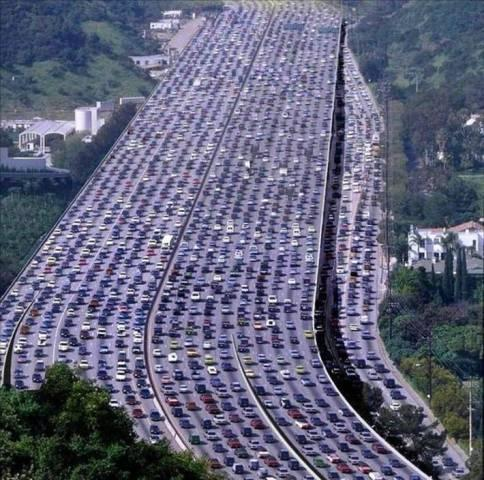
\includegraphics[width=0.7\columnwidth]{images/transito2.jpeg}
	\caption{Imagem do trânsito \cite{autoentusiastasclassic}}.
	\label{fig:transito}
\end{figure}


Segundo o IPEA (Instituto de Pesquisa Econômica Aplicada do Brasil), a mobilidade urbana, nos dias atuais, é um dos principais problemas dos grandes centros. Os reflexos sobre o transporte urbano são evidentes, caracterizados principalmente pelo aumento do tráfego nas vias e consequentemente dos congestionamentos \cite{carvalho2010mobilidade}. Porém, baseado em  \citeonline{gupte2012vehicular}, é possível gerir o tráfego de forma eficiente utilizando redes de veiculos ad-hoc (VANET) de maneira eficiente e autonoma.

Segundo  \citeonline{cavalcanti2008veer}, a crescente quantidade de dispositivos eletrônicos que podem ser embarcados em veículos automotores como DVD, TV, GPS e telefone celular, faz com que os veículos deixem de ser apenas um meio de transporte e passem a oferecer uma rede de serviços e entretenimento para os condutores e/ou passageiros.

%%%%%%      Esse parágrafo ficou pedido
%
%O IEEE (\textit{Institute of Eletrical and Eletronics Enginners}) estabeleceu que a tecnologia  de comunicação utilizada entre veículos, sendo nos Sistemas de Transpote Inteligente ou na comunicação Veículo para Veículo, é derivada do padrao 802.11p, este padrão também conhecido como rede local sem fio cujo espectro de frequência utilizada é na faixa de 5,9 GHz, sendo atribuída numa base hamonizada na Europa, em consonância com atribuições semelhantes no EUA.


%Diante dos desafios encontrados nas redes veiculares, há um grande esforço da comunidade acadêmica em todo o mundo no intuito de saná-los para que seja possível aplicar de maneira segura e estável melhorando a mobilidade urbana nas cidades.
\section{Justificativa, Problemática e Hipótese}

\subsection{Justificativa}

É crescente o número de pesquisas sobre VANETs  com intuito de aumentar a segurança viária, bem como ofertar e comercializar novos serviços a motoristas e passageiros. VANETs que usam veículos como nós móveis, são uma subclasse de rede móveis ad hoc chamadas de MANETs (\textit{Mobile Ad hoc Network}), elas fornecem comunicação entre os veículos próximos e entre veículos  e equipamentos à beira da rodovia mas, aparentemente difere de outras redes por suas próprias características do ambiente. 

Diante da evolução das redes veiculares e da necessidade de garantir o táfego dos dados dentro da alta mobilidade dos nós numa VANET, vê-se a importância de utilizar tecnologias que permitam auxiliar na solução dos principais desafios relacionados a este tipo de rede.  

O uso de VANETs representa uma oportunidade para melhora na segurança, eficiência e conforto relacionados ao trânsito nas grandes cidades, porém, possui características específicas que apresentam obstácolos a serem contornados. 

Os nós numa rede VANET são muito dinâmicos pois os veículos possuem velocidade e direção variável. A alta mobilidade dos nós conduz a uma topologia de rede dinâmica caracterizada pela constante perda de comunicação fazendo com que os algoritmos de roteamentos tornem-se complexos e limitados. Normalmente, VANETs apresentam três aspectos para pesquisas: roteamento, segurança e privacidade, bem como suas aplicações \cite{liang2015vehicular}.

O roteamento em VANETs é baseada na comunicação sem fio e devido à topologia dinâmica e conectividade intermitente, a maioria dos algoritmos em MANETs não estão disponíveis para os vários cenários VANETs, tornando o tema ainda em aberto  e sendo foco de várias pesquisas na atualidade com objetivo de dar confiabilidade na comunicação levando em consideração número de emissores e receptores e tipos de roteamento.

Comentado por \citeonline{cavalcanti2008veer}, os nós de uma rede veicular apresentam como principal caracterista, a alta mobilidade, por serem dinâmicos e apresentarem rápidas variações das condições do meio sem fio são os principais geradores de desafios.  O alto dinamismo representa um contratempo para as comunicações, visto que nem sempre o tempo de contato dos veículos é suficiente para estabelecer uma comunicação efetiva.

Trabalhos como  \citeonline{hadaller2007vehicular}, \citeonline{nandan2005co} e \citeonline{chen2006dynamic}, apresentam propostas que vão desde a implementação de uma infra-estrutura fixa até definir esquemas de agrupamento de nós, visando reduzir a latência de entrega de mensagens para sistemas de segurança. \citeonline{nandan2005co} propuseram uma comunicação eficiente para sistemas P2P com disponibilização de conteúdo utilizando um mecanismo de partição dos arquivos disponíveis em pequenos pedaços.  Este particionamento visa promover uma forma de transferência distribuída,  na qual é possível que um nó esteja recebendo dois pedaços distintos do mesmo arquivo de duas fontes distintas e simultaneamente.  Cabe ressaltar que em grande parte as propostas visam agilizar o processo de transferência de dados em VANETs e implementam mecanismos específicos para minimizar os problemas gerados pela alta mobilidade dos nós.

Dentro desse contexto, este artigo apresenta como principal contribuição, um modelo de arquitetura de software flexível e extensível, que utiliza rede veicular  e  Computação em Nuvem, com a finalidade de proporcionar uma alternativa para os principais desafios relacionados à VANETs tais como: 

\begin{itemize}
	\item{\textbf{meio físico}: interferências devido à prédios,  árvores e outros obstáculos;}
	\item{\textbf{alta mobilidade:} dificulta a troca de informações mais completas; }
	\item{\textbf{topologia}:VANET possui uma característica dinâmica, devido à velocidade que os veículos se movimentam;}	
	\item{\textbf{baixa densidade}: quando a densidade de tráfego é baixa e os veículos estão distantes uns dos outros;}
	\item{\textbf{alta densidade}: muitos veículos em uma pequena área faz com que a quantidade de mensagens trocadas seja um problema;}
	\item{\textbf{segurança}: como as VANETs suportam aplicações de emergência em tempo real e lidam com informações	críticas de segurança no trânsito, estas devem satisfazer os seguintes requisitos de segurança: confidencialidade, integridade, disponibilidade, autenticidade, privacidade e não repudiação para prover segurança na comunicação dos dados \cite{samara2010security} \cite{matos2013analise}.}
\end{itemize} 

Segundo \citeonline{falchetti2015vehicular}, os principais desafios técnicos que são abordadas pela maioria dos pesquisadores, podem ser agrupados em seis categorias: mobilidade, latência, confiabilidade, criticidade(prioridade das mensagens), topologia e segurança. 

Portanto, pesquisar sobre redes veiculares e computação em nuvem, traz a possibilidade de construção de uma plataforma capaz de criar uma VANET virtualizada facilitando a comunicação entre os nós virtuais da rede e simplificando a implementação dos algoritmos de roteamento, segurança e aplicações.

Com o uso da computação em nuvem, os autores  \citeonline{liu2015software} utilizaram um controlador SDN (\textit{Networking Defined Software}) para enviar mensagens para os veículos a partir de um RSU concetados ao controlador, porém, os veículos deveriam pertencer à mesma geolocalização.

Foi criado por \citeonline{hajjidesign} , a plataforma Testbed que serve para testar a implementação real dos roteadores móveis em uma rede veicular virtualizado. A característica principal consiste na sua capacidade em satisfazer ao mesmo tempo as exigências de mobilidade do veículo e o número elástico de roteadores Móveis aplicados.

\citeonline{eltoweissy2010towards} pela primeira vez realizou uma mudança de paradigma imaginado para o ambiente de VANET tradicional para VANET baseado em nuvem. Eles vieram com uma nova noção de VANET chamado AVC (\textit{Autónomas Veiculares Nuvens}).  \citeonline{yan2013security} delineou os desafios de segurança e privacidade nas nuvens veiculares. No entanto, Olariu et ai. discutiu sobre nuvens veiculares de maneira abstrata, sem mencionar uma arquitetura em  particular. 

Recentemente, \citeonline{hussain2012rethinking} propôs três quadros de arquitectura para VANETs baseados em nuvem ou seja VC (\textit{Vehicular Clouds }), VUC (textit{VANET using Clouds)}), e HVC (\textit{Hybrid Vehicular Clouds }) e propôs um esquema conhecido como TIaaS (\textit{Information of traffic as Service}), onde a infraestrutura de nuvem atua para fornecer informações de tráfego para os veículos que se deslocam sobre a estrada.

 \citeonline{qin2012vehicloud} propôs um esquema de roteamento, para VANETs, baseado em nuvem chamado VehiCloud que fornece serviços de roteamento através da infraestrutura de nuvem. Veículos compartilham a sua actual e futuras informações de localização na forma de \textit{waypoints)} com infraestrutura de nuvem e, em seguida, a nuvem lhes proporciona uma melhor informação de roteamento.

De acordo com \citeonline{falchetti2015vehicular}, a integração de VANETs com a nuvem aumenta a utilização das capacidades computacionais que são subutilizados por aplicações de segurança e supera os problemas de roteamento em comunicação V2V (\textit{Vehicle to Vehicle}).

\citeonline{lee2014vehicular} visam interligar recursos OBU (\textit{On Board Unit})e RSU (\textit{Road Side Unit}) em nuvem para tarefas cooperativas sensoriais, de armazenamento e de computação, enquanto outros \cite{hussain2012rethinking} \cite{mershad2013finding} propôem que as RSUs ajam como gateways para as OBUs para acesso às nuvens tradicionais.

Foi proposto por \citeonline{lee2014vehicular} o VCN (\textit{Vehicular Cloud Networking}) que está sendo visto como uma revolução para modernizar a tradicional VANET, que integra informações de redes e Cloud Computing com VANETs tradicionais. No VCN, veículos e  RSU compartilham seus recursos em uma plataforma virtual como ilustrado na figura \ref{fig:vcn}.

\begin{figure} [t]
	\centering
	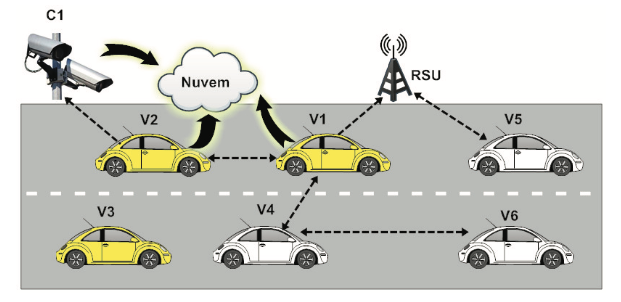
\includegraphics[width=0.7\columnwidth]{images/vcn.png}
	\caption{Modelo do VNC \cite{lee2014vehicular}}.
	\label{fig:vcn}
\end{figure}

%%%%%%%%%% Também ficou solto
%
%Gerla (2012) \nocite{gerla2012vehicular}, introduziu um novo modelo de computação em, o VCC   (\textit{Vehicle Cloud Computing}).  VCC é uma variante do MCC (textit{Movel Cloud Computing}) móvel de computação em nuvem (MCC) \cite{fernando2013mobile}.

\subsection{Problemática}

Como criar uma plataforma em nuvem capaz de permitir a construção de aplicações voltadas para VANETs, considerando o desenvolvimento simplificado e extensível de maneira que o cerne principal da plataforma seja abstraído das novas funcionalidades, mantendo o foco nos principais desafios atualmente encontrados em redes veiculares e permita a escalabilidade. 

\subsection{Hipótese}

Avaliar se o tempo de resposta da arquitetura proposta permite os mais variados tipos de aplicações em VANETs, dada a particularidade deste tipo de rede.

\section{Objetivos da Dissertação}

O objetivo principal desta dissertação é apresentar uma arquitetura de software flexível e extensível, com capacidade de virtualizar nós de uma rede VANET, realizando a comunicação entre os elementos de forma virtual na tentativa de corroborar com a solução de alguns dos principais desafios relacionados à rede veiculares.

\subsection{Objetivos Específicos}
Para acançar a inteção anterior, alguns objetivos específicos devem ser atendidos,  a saber: 
\begin{itemize}
	\item{Projeta uma arquitetura de software de maneira que permita a extensabilidade, flexibilidade e escalabilidade;}	
	\item{Construir a arquitetura utilizando a lingugem Java;}	
	\item{Implementar uma versão para cada camada da arquitetura;}	
	\item{Construir uma aplicação como prova de conceito;}	
	\item{Realizar testes simulados para avaliar seu desempenho e capacidade.}	
\end{itemize} 

\subsection{Metodologia}

No desenvolvimento desta dissertação foram empregadas a pesquisa bibliográfica, pesquisa quantitativa e a pesquisa experimental.

Na pesquisa bibliográfica foi verificado o estado da arte sobre redes veiculares e seus principais desafios. A pesquisa quantitativa foi utilizada para poder quantificar dentre as aplicações relacionadas à VANETs quais os tempos de comunição necessários para viabilidade da solução. E por fim, a pesquisa experimental, pois foram realizados experimentos na arquitetura e gerados dados em um ambiente real para responder a hipótese levantada na problemática.

Na definição do escopo e das metas desta pesquisa, ficou estabelecido definir e construir uma arquitetura de software modular de maneira que cada módulo abstraia detalhes de implementação dos demais, permitindo usufruir de ``contratos'' no uso efetivo dos módulos.

Os cenários para os experimentos foram definidos utilizando movimentações reais dentro da cidade de Aracaju-Sergipe Brasil, os quais foram extraídos, 12 milhoes de movimentações,  de uma empresa de taxi .

Para alcançar os resultados foi necessário estabelecer conexões entre os nós de uma rede VANETs, permitindo a criação de rede de maneira dinâmica, ``aleatória'' e mantendo a integridade dos dados.

A métrica e a técnica de avaliação desta pesquisa foi o tempo de processamento de cada mensagem enviada ao servidor como também o tempo de comunicação entre os veículos e os servidores em nuvem contrapondo entre as velocidades do 2G, 3G, 4G e 5G, permitindo avaliar se as velocidades atuais da telefonia móvel suportam a solução e um teste de carga para medir a capacidade operacional da plataforma.
 
%Para execução da simulação com dados reais, foi constuído uma aplicação que conectava ao servidor em nuvem e realizava as devidas transmissões, sendo que as coordenadas vinham de um arquivo
\subsection{Contribuições}

A computação veicular em nuvem é um novo campo de pesquisa com o potencial de mudar a vida das pessoas. Ele  traz a eficiência, segurança e conforto para motoristas e passageiros \cite{falchetti2015vehicular}. Sendo a principal contribuição deste trabalho a construção de uma arquitetura para criação de redes veiculares em nuvem como também a análise dos dados coletados a partir dos experimentos. Nesse sentido, este estudo mostra que também é válido o uso de VCN no auxílio das soluções para os principais desafios relacionados à VANETs.

Outra contribuição importante foi poder instalar e analisar aspectos de segurança nas redes veiculares podendo apenas assinar a mensagem ou criptografá-la, seguindo com análise de viabilidade de ambos os casos. Conclui-se que o desempenho e eficiência da arquitetura atendem aos requisitos relacionados à VANETs. E assim, demonstrar que o tempo de conexão e processamento em uma rede VCN em ambiente de simulação atende às necessidades de vários tipos de aplicações relacionadas a VANETs.

Dentro desse contexto, este rabalho apresenta como principal contribuição, um modelo de arquitetura de software flexível e extensível, que utiliza rede veicular ad-hoc (VANET) e  Computação em Nuvem, com a finalidade de proporcionar uma alternativa para os principais desafios relacionados à VANETs .


\section{Organização do Trabalho}
%Antes do penúltimo parágrafo, inserir um parágrafo contendo as principais contribuições do artigo. Por exemplo: The main contributions of this work are ?.. X Y Z.
Os demais capítulos da dissertação estão organizados da seguinte forma:
O capítulo 2 aborda de maneira geral, conceitos de internet das coisas, sistemas distribuiídos e as redes veiculares e suas aplicações. No capítulo 3 é apresentado a arquitetura I9Vanet, seus módulos e detalhes da tecnologia utilizada na construção. Já o capítulo 4, apresenta o processo de avaliação realizado na arquitetura I9Vanet bem como a análise dos resultados.
O capítulo 5 apresenta as conclusões, destacando as principais contribuições, o resultado da análise dos dados e sugestão para os possíveis trablahos futuros.

%\chapter{Redes Veiculares}\label{sec:vanet}

\chapter{Rede de Sensores sem Fio}
%As redes de sensores sem fio ou WSN (\textit{Wireless Sensor Network}), visa resolver um conjunto de problemas, contudo, além das tarefas de monitoramento, a WSN projetou-se para solução de diversos tipos de aplicações. 

As Redes de Sensores ou WSN (\textit{Wireless Sensor Network}) estão emergindo como uma nova ferramenta para aplicações importantes em diversos campos como vigilância militar, monitoramento de ambiente,  e coleta de informações em ambiente hostil, vigilância de edifícios, entre outros. 

\section{Definição}
Uma rede de sensores sem fio é uma tecnologia específica que ajuda na criação de aplicações com foco em cidades inteligentes. O seu objectivo consiste em criar uma rede que contenha muitos nós de sensores ``inteligentes'' que possam detectar múltiplos parâmetros de interesse para uma melhor gestão da cidade.

Para realizar tarefas de detecção, a maioria dos Sistemas de Transporte Inteligentes (ITS) atuais contam com sensores caros, que oferecem apenas funcionalidade limitada. Uma tendência mais recente consiste em utilizar WSN para tal finalidade, o que reduz o investimento necessário e permite o desenvolvimento de novas aplicações colaborativas e inteligentes que contribuem ainda mais para melhorar tanto a segurança de condução como a eficiência do tráfego \cite{losilla2011comprehensive}.

Da mesma forma que em redes de sensores sem fio, os nós de uma rede VANET necessitam trocar informações com outros nós próximos o que torna técnicas de WSN aplicáveis à redes veiculares entretanto, há o desafio da alta mobilidade dos nós em uma rede VANET.

% e um controle do tráfego urbano. Cada nó de rede esgota sua energia porque a capacidade da bateria é limitada. Neste trabalho, propomos estudar o problema das redes de sensores sem fio em cidades inteligentes, com foco em baixo custo e economia de energia. É necessário estudar a arquitetura de um nó sensor que se caracteriza por uma capacidade de energia limitada, tornando a otimização do consumo de energia na rede a principal restrição para prolongar a vida útil da rede. Vamos discutir os diferentes fatores envolvidos no consumo de energia e vamos apresentar algumas técnicas para preservá-lo. Neste trabalho, apresentaremos uma visão geral de nossa solução para a conservação de energia na WSN. Vamos descrever a nossa solução que visa evitar pacotes de transmissão freqüentes de dados enviados para o controlador de luz. Então, vamos detalhar os dois simuladores (GLD e SUMO) que usamos. Resultados de simulação têm mostrado que a nossa solução permite a minimização do número de pacotes enviados, e, portanto, reduzir o consumo de energia, além disso, uma vida útil da rede será maior.

%Antes de entender o que é uma RSSF precisamos saber o que é uma rede Ad-Hoc. As redes Ad-Hoc não dependem de infraestrutura pré-definida, não há uma topologia e é descentralizada (veremos mais a frente que, dependendo do protocolo de roteamento e da aplicação, uma rede Ad-Hoc pode se tornar centralizada). Nesse tipo de rede, os nós se comunicam diretamente por um meio físico. Essa conexão dinâmica permite que os nós entrem e saiam da rede sem afetar seu funcionamento.

%Dizemos que, numa rede Ad-Hoc, cada nó é responsável pela retransmissão das mensagens. Uma característica interessante é que a rede pode ser formada por diferentes tipos de nós, desde que todos apresentem as características acima. Se os nós são dispositivos móveis, especificamos a rede Ad-Hoc como MANET (Mobile Ad-Hoc Network).

\section{Arquitetura de Rede e Topologia}

Uma aplicação ITS baseada em WSN distribuída, realiza quatro tarefas principais distintas: (i) aquisição de informação, (ii) distribuição de dados, (iii) processamento de dados para planejar as ações necessárias e, finalmente, (iv) execução das ações apropriadas  \cite{losilla2011comprehensive} . Uma vez que estas tarefas podem ser realizadas de forma independente, pode considerar-se que definem correspondentemente quatro subsistemas diferenciados que estão presentes nos sistemas ITS, como mostrado na figura \ref{fig:arquiteturas_its_wsn}, nomeadamente o subsistema «Sensores», o subsistema «Distribuição», o subsistema «Tomada de decisões» e o subsistema «Execução». 

\begin{figure} [t]
	\centering
	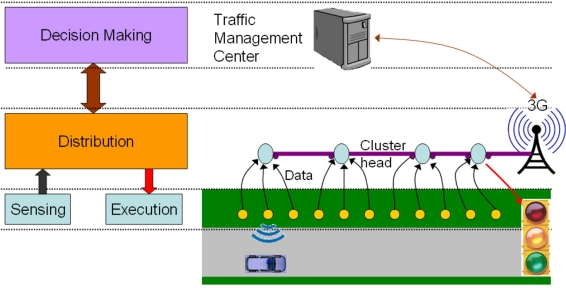
\includegraphics[width=0.8\columnwidth]{images/camadas_wsn.jpg}
	\caption{Arquitetura de referência para aplicações ITS baseadas em WSN. \cite{losilla2011comprehensive}}.
	\label{fig:arquiteturas_its_wsn}
\end{figure}

\subsection{Subsistema de Sensores}

Este subsistema é composto pela aquisição das informações relevantes, principalmente em relação ao tráfego e estados da rodovia. Numa aplicação ITS baseada em WSN, não necessariamente todos os dispositivos utilizam a tecnologia WSN, permitindo uma distribuição de tarefas entre dispositivos que utilizam tecnologias diferentes. A implantação do subsistema de sensores consiste na implantação de um ou mais WSNs em toda a área de observação (estradas ou parques de estacionamento), que detectam veículos através dos seus sensores e, opcionalmente, comunicam-se sem fios com eles. Os nós WSN são divididos em grupos seguindo um esquema semelhante, e a implantação consiste em uma composição, tipicamente homogênea, desses grupos de nós. Portanto, eles podem ser considerados como os blocos de construção do subsistema de detecção. Deve-se notar que, além disso, os nós que formam esses blocos podem propagar informações dentro deles, mas isso não deve ser confundido com o subsistema de Distribuição. A propagação de dados no subsistema de sensores é restrita a áreas locais, visando extrair informações do bloco / grupo (para um nó coletor) ou ativar o processamento colaborativo com nós próximos. Se for necessária a disseminação de dados através de áreas maiores, é necessário o uso do subsistema de distribuição.
\subsection{Subsistema de Distribuição}

O subsistema de distribuição é responsável pela troca de informações entre os diferentes subsistemas de uma aplicação ITS. Numa arquitectura em camadas tal como a da Figura \ref{fig:arquiteturas_its_wsn}, ela é colocada numa posição central, recebendo pedidos de comunicação de todos os outros subsistemas e servindo-os em conformidade. É responsável pela transmissão dos dados detectados para o subsistema «tomada de decisões» e, por outro lado, pela transmissão de comandos do subsistema «tomada de decisões» para os subsistemas «detecção e execução» \cite{sung2007collision}. Da mesma forma, interconecta os diferentes gruposde sensores de uma rede. Isso resulta em uma rede escalável criada pela composição desses grupos. A este respeito, o subsistema de distribuição pode igualmente interligar grupos fisicamente isolados de nós ou veículos, permitindo assim a interconexão de ilhas WSN desdobradas em diferentes partes ao longo da estrada \cite{weingartner2007prototype} ou de agrupamentos de veículos que de outra maneira formariam VANETs não ligados \cite{tripp2010performance} .

O subsistema de distribuição consome uma quantidade significativa de energia devido às exigências impostas aos seus dispositivos. Eles são encarregados de encaminhar cada evento relatado por cada nó do subsistema de sensores, que pode ocorrer em uma alta taxa de frequência. Além disso, deve ser feito sob as restrições de tempo definidas pela aplicação. Isto requer nós muito ativos para garantir a entrega de informações em tempo hábil, comprometendo a economia de energia. Portanto, os dispositivos usados neste subsistema precisam de um orçamento de energia mais generoso do que os nós de sensores, tornando necessárias fontes de energia adicionais \cite{losilla2011comprehensive}.

Existem diferentes formas de implementar o subsistema de distribuição. Uma delas consiste em empregar redes veiculares para disseminar informações. Dispositivos utilizados nos veículos não têm restrições de energia, uma vez que podem ser alimentados por instalações do próprio veículo. Além disso, a mobilidade de veículos, que é um fator limitante para outros tipos de aplicações, ajuda a espalhar dados em veículos e nós estáticos ao longo da rodovia, e alivia os nós estáticos das tarefas de distribuição. O esquema mais simples envolve a utilização de transmissão directa entre veículos, isto é, uma rede de um salto que permite a partilha de dados de um veículo de origem para cada veículo que se aproxima \cite{li2007snms} \cite{miura2006evaluation}. A segunda alternativa baseia-se na utilização de uma rede de distribuição VANET multi-salto \cite{qin2010integrated}. Esta opção requer mais recursos do sistema, mas também facilita a disseminação mais rápida de dados e escalas muito melhor à medida que o número de veículos tecnologicamente equipados cresce.

De acordo com \citeonline{losilla2011comprehensive}, um subsistema de distribuição baseado em redes celulares é uma opção atraente, não apenas por sua alta disponibilidade, mas também pelo custo de implantação. Mesmo gateways são dispositivos caros que requerem interfaces de rede celular, apenas alguns deles são necessários para serem colocados perto de estações de base celulares (BS) e alguns nós mais baratos que conectam os nós de detecção com os gateways devem ser implantados. Por outro lado, os custos de exploração também devem ser levados em conta, uma vez que os operadores celulares cobram a utilização da BS. Isso pode levar a uma outra escolha, quer quando não está planejado para pagar o uso de BS ou não estão disponíveis, que consiste em usar IMS (Internet Multimedia Subsystems) \cite{birk2009iroad} que fornecem acesso ao Sistema de Distribuição através de diferentes tecnologias (2G, 2.5G, 3G, 4G, 5G, WLAN) independentemente do operador.

\subsection{Subsistema de Tomada de Decisão}
Subsistema de tomada de decisão é também conhecido por DMS (\textit{Decision Making subsystem}), é responsável pelo planejamento das ações necessárias para alcançar os objetivos do sistema. As tarefas atribuídas a este subsistema podem ser divididas em três grupos diferentes. O primeiro deles inclui tarefas destinadas ao armazenamento e ao pré-processamento de dados. Trata-se da enorme quantidade de dados que chega ao subsistema, filtrando e armazenando apenas informações relevantes e subseqüentemente acessando-a. O segundo grupo trata as informações de tráfego de diferentes fontes e as processa de acordo com o objetivo da aplicação. Finalmente, o terceiro grupo de tarefas é responsável por endereçar comandos de controle, bem como para gerenciamento da rede.

O DMS pode ser executado em diferentes níveis. Em um nível superior, ele pode ser implementado em centrais de monitoramento de tráfego. Isto implica que todos os dados recolhidos pelo subsistema de sensores são enviados, através do subsistema de distribuição, para o DMS, que deve suportar um fluxo de dados assimétrico. A principal vantagem desta abordagem é a possibilidade de realizar cálculos complexos sobre uma grande quantidade de informação. Inversamente, se apenas o processamento simples for aplicado, o DMS pode ser distribuído entre os nós . Isso permite executar algoritmos colaborativos simples entre nós vizinhos que permitem a execução de aplicações de segurança de tráfego em tempo real. Finalmente, uma outra solução é a utilização de dispositivos inteligentes (smartphones, etc.) em veículos, que podem receber dados brutos de redes rodoviárias e usá-los, por exemplo, para planejar rotas \cite{losilla2011comprehensive}.

\subsection{Subsistema de Execução}

Este subsistema é responsáve por executar ações necessárias que promovam mudanças no fluxo de tráfego de acordo com o objetivo da aplicação ITS. É composto principalmente por dispositivos que fornecem estímulos visuais e acústicos aos condutores, embora outros destinados à automação de veículos também pertençam a este subsistema. Podem ser utilizados equipamentos diferentes. Os semáforos ou os sinais de mensagem variável instalados ao longo das estradas são opções atrativas que proporcionam um controlo rigoroso e adaptabilidade a diferentes situações, respectivamente. Eles oferecem a vantagem de serem infra-estruturas rodoviárias amplamente adotadas, adequadas para reutilização em aplicações para ITS, o que ajudaria a reduzir os custos de implantação \cite{losilla2011comprehensive}. 

O emprego de sistemas no veículo oferece, por um lado, a possibilidade de apresentar informação personalizada para cada veículo e, por outro lado, a possibilidade de utilizar sinais acústicos e mensagens que diminuem as distracções durante a condução. Além disso, as informações provenientes dos sistemas rodoviários podem ser integradas nos sistemas de informações no veículo, o IVI (\textit{In-Vehicle Infotainment}), por exemplo, para a sua fusão com mapas digitais ou outros serviços de informação (horários de transporte, previsões meteorológicas, etc.). Atualmente, o número considerável e crescente de smartphones, navegadores ou tablets abre o caminho para a adoção de sistemas dentro do veículo. No entanto, há um interesse crescente dos fabricantes de veículos em incorporar sistemas IVI em seus produtos como um diferencial competitivo. A este respeito, novos modelos de automóveis de empresas importantes estão equipados com sistemas como o iDrive da BMW \cite{niedermaier2009new}, o Audi MMI [44], a Ford SYNC [45] ou GENIVI Apollo da aliança GENIVI apud  \citeonline{losilla2011comprehensive}, que visam facilitar o desenvolvimento Das aplicações IVI.


%Nesse trabalho, vamos apresentar as Redes de Sensores Sem Fio. Primeiramente, tentaremos mostrar os problemas que motivaram sua criação e, depois, tentar entender seu funcionamento de modo geral através de uma abordagem mais técnica. Por fim, veremos algumas aplicações e analisaremos as tendências para esse tipo de rede.
\chapter{Sistemas Distribuídos}

%Os sistemas distribuídos é de suma importância para que se possa atender a uma crescente demanda de usuários o que seria 
Com o surgimento das redes locais (LAN), o homem tenta aproveitar melhor o proder computacional dividindo tarefas em vários computadores para realizar processamento paralelo de modo a aumentar o poder computacional sem utilizar super computadores. Surgindo assim, o conceito de sistemas distribuídos (SD).

\section{Definição}

De acordo com \citeonline{distribuidos2007principios}, um sistema distribuído é um conjunto de computadores independentes entre si, que se apresenta a seus usuários como um sistema único e coerente. Já  \citeonline{coulouris2013sistemas}, define sistemas distribuídos como sendo uma coleção de computadores autônomos interligados através de uma rede de computadores e equipados com software que permita o compartilhamento de hardware, software e dados.

De acordo com as definições, os sistemas distribuídos apresentam algumas caracterísitas: concorência de recursos,  falta de um relógio e falhas de componentes independentes. Sendo o compartilhamento de recursos um dos principais motivos para se utilizar sistemas distribuídos. 

Os desafios atrelados à construção de sistemas distribuídos são: a heterogeneidade de seus componentes, ser um sistema aberto, segurança e escalabilidade, tolerância a falhas, a concorrencia aos recursos e a transparêcia \cite{coulouris2013sistemas}.

A miniaturização dos dispositivos  e a interligação em redes sem fio, tem ocasionado uma convergência de equipamentos cada vez menores com sistemas distribuídos. A portabilidade desses dispositivos, torna a computação móvel possível e fundamental para que a computação ubíqua ou pervasiva, seja utilizada cada vez mais pelo usuário e de maneira transparente e natural.

\section{Características e Desafios}

Os sistemas distribuídos é encontrado em toda parte, contudo, há desafios que todo sistema SD precisa se preocupar tais como: heterogeneidade, sistemas abertos,  segurança, escalabilidade e tolerância a falhas.

\subsection{Heterogeneidade}

Segundo \citeonline{coulouris2013sistemas}, os aspectos que devem ser levados em consideração pela heterogeneidade, estão relacionados à rede, hawdare, sistemas operacionais, linguagens de programação e implementações.

\subsection{Sistemas Abertos}

Um sistema é considerado aberto, quando é possível estendê-lo de várias maneiras. O fato de um SD ser ou não um sistema aberto é determinado pelo grau com que os novos serviços podem ser inseridos para uso por uma variedades de aplicações clientes \cite{coulouris2013sistemas}.

Para que um sistema seja considerado aberto, é necessáio publicar as principais interfaces dos componentes de software. Entretanto, a publicação do padrão de comunicação com o software é apenas o início para adicionar novos serviços a um sistema distribuído.

\subsection{Seguança}

A segurança atrelada à sistemas distribuídos possui três componentes são eles: confidencialidade, integridade e disponibilidade. O primeiro ítem, deve proteger o acesso à informação de pessoas não autorizadas. Quanto à integridade, os sistemas distribuídos devem garantir a não adulteração dos dados e por último, a disponibilidade, o qual deve proteger contra interferência de acesso ao recurso.

\subsection{Escalabilidade}

Em se tratando de escalabilidade, há dois tipos: a vertical e a horizontal, sendo a primeira, a forma de escalonar um sistema centralizado, realizando um \textit{upgrade} na memória, nos processadores e/ou nos discos, quando possível. Já no escalonamento horinzontal, consiste em acoplar mais máquinas em um ambiente distribuído, não havendo limites.

Um dos grandes objetivos dos sistemas distribuídos, é permitir o aumento de capacidade à medida que cresce a demanda pelo recurso. E os principais desafios é balancear os custos dos recursos físicos com a perda de desempenho, impedindo que os recursos de software se esgotem evitando gargalos na performance. Sendo assim, a escalabilidade é considerada um tema central em sistemas distribuídos.

\subsection{Tolerância a Falhas}

Infelizmente os sistemas de computador falham, seja por motivo de hardware ou software, os programas podem produzir resultados incorretos. Em um ambiente com sistema distribuído, alguns componentes podem falhar equanto outros continuam funcionando, sendo cosiderado algo complexo tratar corretamente cada problema que pode ocorrer. A tolerância a falhas é fundamental para o bom funcionamento das aplicações de segurança crítica \cite{gorender2002modelo} . Dentre as técnicas para tolerância a falhas temos: 

\begin{itemize}
	\item{\textbf{Detecção de Falhas}: algumas falhas podem ser detectadas antes que mesmo que afete o sistema. Para isso, somas de verificação podem ser utilizadas para verificar a integridade da informação por exemplo, mas outras falhas não há como prevê, como, por exemplo, a parada de um servidor.} 	
	\item{\textbf{Mascaramento de Falhas: } algumas falhas podem ser mascaradas, por exemplo, a lentidão momentânia de um \textit{link} pode ser resolvido retransmitindo novamente a mensagem, sem precisar que o usuário tome conhecimento.}
	\item{\textbf{Recuperação de Falhas: envolve desenvolver softwares capazes de recuperar ou retroceder o estado dos dados para um momento consistente.}}
	\item{\textbf{Redudancia:} alguns serviços podem melhorar sua tolerancia a falhas com o uso de discos espelhados ou \textit{links} de Internet duplicados, entre outras redundancias, assim, caso algum destes recursos falhem, terá uma alternativa para continar funcionando.}
\end{itemize} 

\subsection{Transparência}

A transparência tem como objetivo, esconder, do usuário ou programador, detalhes da separação dos componentes em um sistema distribuído, de maneira que seja percebido como um todo.

%Em um ambiente de redes veiculares em nuvem, é fundamental o uso de sistemtas distribuídos para que se consiga atender à demanda, permitindo a escalabilidade.

\section{Comunicação em Sistemas Distribuídos}

As restrições temporais determinam a variação dos modelos de sistemas distribuídos existentes. Podendo ser síncronos ou assíncronos. O modelo síncrono deve ser utilizado quando se conhece os limites temporais, permitindo que haja uma estimativa com relação ao tempo de execução dos protocolos do sistema e funções  da própria aplicação distribuída \cite{lamport1982byzantine} \cite{lynch1996distributed} \cite{cristian1991reaching}. A tolerância a falhas é mais eficiente com a comunicação síncrona, pois permite o uso de \textit{timeout} mais facilmente. Entretanto, nos sistemas assíncronos (\textit{time free}), não há restrições temporais, sendo impossível obter o consenso  na presença de falhas \cite{fischer1985impossibility} \cite{de2000failure}, devido à dificuldade inerente desse tipo de sistema em diferenciar entre uma operação com falha ou extremamente lenta \cite{gorender2002modelo}.

Os modelos de comunicação existentes para sistemas distribuídos, baseiam-se ou nas características sincronas de redes locais ou em ambientes de melhor esforço como os da Internet \cite{gorender2002modelo}. Nenhum dos modelos consideram as arquiteturas IntServ e DiffServ para prover controle de QoS (Qualidade de serviço).

As arquiteturas IntServ e DiffSer foram propostas pela IETF (\textit{Internet Engineering Task Force}) cujo objetivo  é permirtir que sistemas de comunicação possam fornecer serviços com diferentes níveis de qualidade, levando em consideração aspectos como: fixação de limite para transferência de dados e diferentes prioridades com relação à possibilidade de perda de pacotes.

\subsection{Comunicação Cliente-Servidor}

A comunicação baseada no Cliente-Servidor foi projetada para suportar a troca de mensagens em interações tipicamente síncronas, pois o processo no cliente bloqueia a execução até a chegada da resposta. Também é considerada confiável, já que a resposta é a confirmação da chegada da requisição no servidor \cite{coulouris2013sistemas}.

O protocolo utilizado na comunicação Cliente-Servidor, é basedo em três primitivas de comunicação: \textit{doOperation}, \textit{getRequest} e \textit{sendReply}. A maioria dos sistemas RMI (Remote Mehthd Invocation)e RPC (\textit{Remote Procedure Call}).

O método \textit{doOperation} é utilizado para invocar processos remotos. Seus parâmetros especificam  o objeto remoto e a operação a ser executada. A segunda primitiva, o \textit{getRequest}, é executado por um processo no servidor, para ler as requisições do serviço. Após execução do processo, pelo servidor, será executado o \textit{sendReply} para enviar a mensagem de resposta para o cliente, fazendo com que o método \textit{doOperation} seja desbloquedo liberando da aplicação cliente.

\subsection{Comunicação em Grupo}

Para fornecer tolerância a falhas à disponibilidade, é necessário o uso de difusão seletiva (\textit{multicast}) em situações que precise realizar uma comunicação de um processo com um grupo de processos.

A troca de mensagem \textit{multicast} fornecem uma infra-estrutura importante para construção de sistemas distribuídos com as seguintes características:

\begin{itemize*}
	\item{Tolerância a falhas baseada em serviços replicados: as requisições do cliente são solicitadas para todos os membros do grupo onde cada um é responsável por executar a mesma operação. Mesmo se algum requisição falhar, o cliente pode ser atendido.}
	\item{Localizar servidores na interligação em rede espontânea: mensagens \textit{multicast} podem ser utilizadas para localizar os serviços de descobertas disponíveis, podendo ser usadas por servidores e clientes.}
	\item{Melhor desempenho através da replicação de dados: em alguns casos, os dados são replicados nas máquinas dos clientes, e quando houver mudança, a atualização é feita por \textit{multicast}.}
	\item{Propagação de notificações de um evento: pode ser utilizado para notificar um grupo, de servidores ou clientes, quando ocorrer mudanças em um determinado evento.}
\end{itemize*}


\subsection{Protocolos de Comunicação}

Há diversos estilos de empacotamento para troca de mensagens em sistemas distribuídos. O CORBA, opta por empacotar os dados para uso pelos destinatários que já conhecem seus tipos anteriormente. Ao contrário do Java, que serializa os dados incluindo informações completas sobre os tipos de seu conteúdo, possibilitando que o destinatário possa reconstruí-los. A linguagem XML segue o modelo semelhante à do Java, fornecendo os tipos de seus conteúdos. 

A figura \ref{fig:estrutura_comunicacao} mostra os mecanismos usados para criação de clientes e servidores para \textit{WebService}, CORBA e Java-RMI. Quando são utilzados stubs gerados automaticamente no lado do cliente para Web Services, os processos de desenvolvimento e a complexidade do código para o cliente e do servidor, são praticamente os mesmos para soluções Web Service, Java-RMI e CORBA. Os fatores que determinarão a escolha serão: a interoperabilidade e o desempenho \cite{gray2004comparison}. Sendo que os Serviços Web permite uma maior integração entre plataformas distintas e dispositivos, enquanto que o desempenho favorecerá ao CORBA e Java-RMI. 

\citeonline{gray2004comparison} realizou um experimento que enviava uma única solicitação de dados e encerrava. Em qualquer dos três casos, \textit{Web Services}, CORBA e Java-RMI, as tecnologias de serviços da Web funcionam bem em comparação com as outras duas, como mostra a tabela \ref{tbComparacaoWS_CORBA_RMI}.

\begin{table}[!h]
	\centering
	\caption{Análise de custos de solicitação de uma única requisição utilizando várias tecnologias\cite{gray2004comparison} }
	\label{tbComparacaoWS_CORBA_RMI}
%	\begin{tabular}{|p{3.0cm}|p{3cm}|p{2.5cm}|p{3.0cm}|}
	\begin{tabular}{|l | c|c|c|}
		\hline
		\rowcolor[gray]{0.7}
		Tecnologia & Latência Total  & Total Pacotes  & Total Dados Transferidos (B)  \\ \hline
		WS              & 0,11s & 16 & 3338  \\ \hline
		CORBA        & 0,48s & 8 & 1111  \\ \hline
		Java-RMI     & 0,32s & 48 & 7670  \\ \hline
	\end{tabular}
\end{table}

%Normalmente, um começa com uma definição de interface para o serviço. Um stub do lado do cliente é gerado automaticamente a partir desta interface. No lado do servidor, a interface é processada para render uma classe base para a classe de implementação que deve ser escrita pelo desenvolvedor. Com os mecanismos e os custos do desenvolvimento sendo muito semelhantes, outros fatores determinarão a escolha de uma solução técnica. Os desenvolvedores de sistemas terão que escolher entre interoperabilidade onde os Serviços da Web têm vantagens e desempenho que favorecerá o Java RMI ou o CORBA.

\begin{figure} [t]
	\centering
	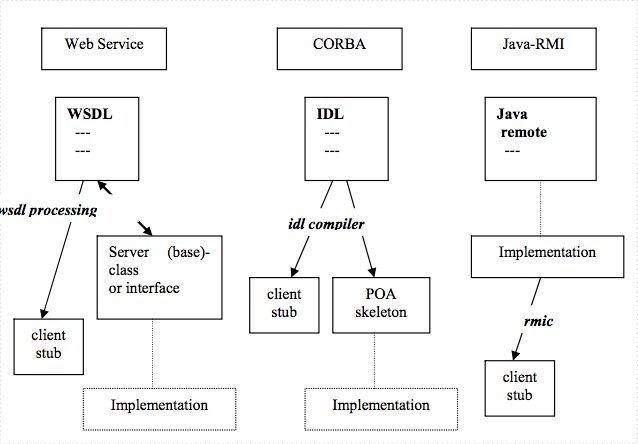
\includegraphics[width=0.8\columnwidth]{images/estrutura_comunicacao.png}
	\caption{Geração de componentes de cliente e servidor, a partir da interface para Web Services, CORBA e Java-RMI \cite{gray2004comparison}}.
	\label{fig:estrutura_comunicacao}
\end{figure}


\subsubsection{WebSocket}

A tecnologia \textit{websocket} foi introduzida pelo HTML5 (\textit{HyperText Markup Language} quinta geração) através da RFC 6455: \textit{The WebSocket Protocol}, o qual permite utilizar um canal de comunicação bidirecional entre um cliente e um servidor remoto, de forma persistente e dedicado usando um único \textit{socket} TCP. Isto é, a comunicação pode ocorrer nos dois sentidos simultâneo e assincrono e a conexão permanece aberta até que em uma das partes realize o fechamento \cite{melnikov2011websocket}.

O \textit{WebSocket} é um protocolo que é definido na camada de aplicação e pode ser utilizado para superar restrições existentes na camada de transporte. Utiliza o modelo de mensagens cliente-servidor como base e suporta tanto dados binários quanto texto simples \cite{themudo2014implementaccao}.

As fases de conexão \textit{WebSocet} estão representadas na figura \ref{fig:etapas_ws}, que vai da criação do canal TCP, depois, troca de mensagens e por último, o fechamento. Na fase de \textbf{Ligação \textit{WebSocket}} é realizada a troca de mensagens indefinidamente.

\begin{figure} [h]
	\centering
	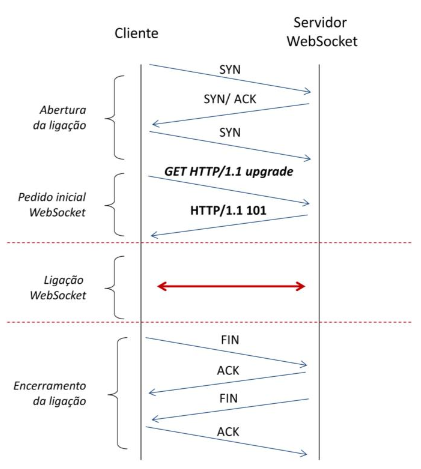
\includegraphics[height=8cm]{images/etapas_ws.png}
	\caption{Etapas de uma conexão \textit{WebSocket} \cite{themudo2014implementaccao}}.
	\label{fig:etapas_ws}
\end{figure}



\chapter{Redes Veículares}


\section{Definição}

As VANETs que usam veículos como nós móveis são uma subclasse de rede móveis ad hoc chamadas de MANETs. Elas fornecem comunicação entre os veículos próximos e entre veículos e equipamentos à beira da rodovia. Os nós numa rede VANET são muito mais dinâmicos, pois os veículos possuem velocidade e direção variável. A alta mobilidade dos nós conduz a uma topologia de rede dinâmica caracterizada pela constante perda de comunicação \cite{bubenikova2014security} \cite{jakubiak2008state}. E podem ser categorizadas segundo o tipo de ligações existentes. Dessa maneira, consideremos as treis artuiteturas de reces veículares \cite{luis2009melhoria}, como mostra a figura \ref{fig:arquiteturas_vanets}: 


\begin{itemize}
	\item{\textbf{Arquitetura WLAN ou celular:} baseada na utilização de antenas fixas, colocadas ao longo da rodovia funcionando como pontos de acesso à rede. Não existe qualquer ligação direta entre os veículos. Em uma cenário de auto-estrada, a implantação dos equipaentos à beira da rodovia de maneira suficiente para permitir a cobertura necessária pode tornar uma solução bastante dispendiosa.}	
	\item{\textbf{Arquitetura ad-hoc:} é considerada uma arquitetura ad-hoc quando não há quaisquer uso de infra-estruturas para realizar a comunicação, sendo as ligações é feita diretamente entre os nós envolvidos. Fatores como velocidade ou densidade dos nós podem pôr em \textit{check} o desempenho deste tipo de rede.}	
	\item{\textbf{Arquitetura híbrida: } tem objetivo de retificar as falhas existentes nas duas arquiteturas anteriores, utilizando concomitatemente as arquiteturas ad-hoc e WLAN}	
\end{itemize} 


\begin{figure} [t]
	\centering
	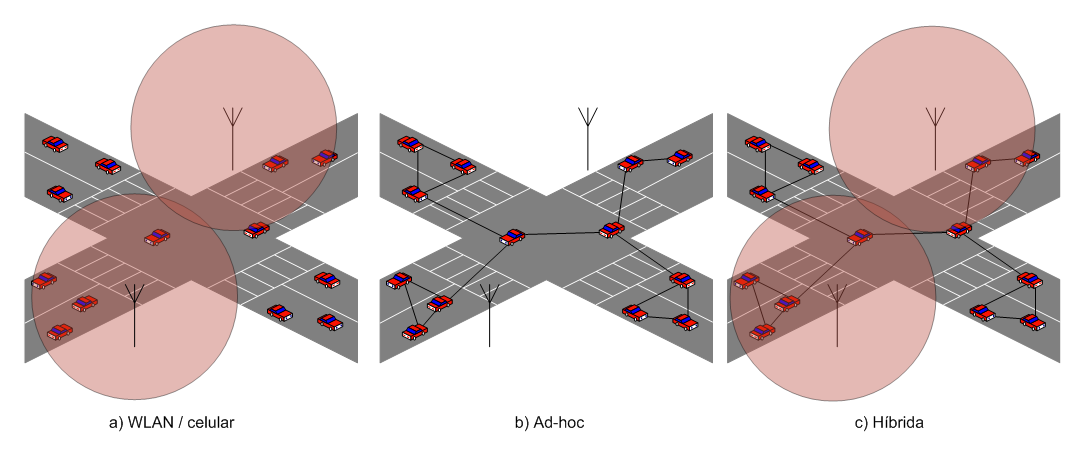
\includegraphics[width=0.8\columnwidth]{images/tipos_arquiteturas_vanets}
	\caption{Arquiteturas de redes veiculares\cite{luis2009melhoria}}.
	\label{fig:arquiteturas_vanets}
\end{figure}


As comunicações em VANETs são categorizadas em 4 tipos:
\begin{itemize}
	\item {Em veículos: pode ser utilizado para detectar a fadiga e/ou sonolência de um motorista que representa  risco na segurança;}
	\item {Entre veículos: a comunicação V2V (veículo para veiculo) pode fornecer uma plataforma de intercâmbio de dados para compartilhamento de informações de advertência de modo a alertar o motorista;}
	\item {Entre veículos e rodovia (V2I): permite atualização em tempo real do tráfego e fornece detecção e monitoramento do ambiente;}
	\item {Entre veículo e nuvem: os veículos podem comunicar-se através da banda larga sem fio tais como 3G, 4G ou WIMAX podendo enviar dados para uma central, o que permitiria um controle mais abrangente do tráfego e assistência ao motorista}
\end{itemize}


As aplicações VANETs podem ser divididas em 3 classes: segurança, entretenimento e assistência ao motorista. O principal desafio relacionado à segurança, está ligado à velocidade de alerta ao condutor, para que possa ter tempo hábil de reação. Nas aplicações de entretenimento, destacam-se os sistemas de compartilhamento de conteúdo e jogos. Já sobre a assistência ao motorista, são aquelas que auxiliam o condutor como por exemplo, através do uso de informações sobre as condições do trânsito \cite{souzasoaressbrc}.

\section{Características e Desafios}

%As redes veiculares ad-hoc caracterizam-se por serem redes sem fio em que todos os nós são efetivamente ativos na comunicação, ou seja, não necessitam de uma infraestrutura fixa de centralização.

Como mensionado anteriormente, as redes veiculares apresentam como principal caracteristica a sua alta mobilidade e é justamente por isso que surge uma série de desafios a serem tratados. Dentre os maiores desafios encontram-se:

\begin{itemize}
	\item{\textbf{meio físico}: interferências devido à prédios,  árvores e outros obstáculos;}
	\item{\textbf{alta mobilidade:} dificulta a troca de informações mais completas; }
	\item{\textbf{topologia}:VANET possui uma característica dinâmica, devido à velocidade que os veículos se movimentam;}	
	\item{\textbf{baixa densidade}: quando a densidade de tráfego é baixa e os veículos estão distantes uns dos outros;}
	\item{\textbf{alta densidade}: muitos veículos em uma pequena área faz com que a quantidade de mensagens trocadas torne-se um problema;}
	\item{\textbf{segurança}: como as VANETs suportam aplicações de emergência em tempo real e lidam com informações	críticas de segurança no trânsito, estas devem satisfazer os seguintes requisitos de segurança: confidencialidade, integridade, disponibilidade, autenticidade e não repudiação para prover segurança na comunicação dos dados \cite{samara2010security} \cite{matos2013analise}.}
	
\end{itemize} 

Cada um dos desafios relacionados está sendo tratado na arquitetura I9Vanet, uma vez que o objetivo da arquitetura é justamente ajudar a resolver tais problemas.


\section{Segurança}

Dito por \citeonline{wanghamsegurancca}, a segurança em redes veiclares é um fator crucial que precisa ser levado em consideração, pois a falta desta pode afetar a vida das pessoas. Como quaisquer redes de computadores sem fio e redes \textit{ad-hoc}, estas estão sensíveis a ataques, tais como: 	negação de serviço, alteração de mensagens \cite{raya2006securing}.

Para construir uma arquitetura de segurança robusta para redes veiculares, é necessário estudar as peculiaridades dos ataques que podem ocorrer. Do memso modo que as redes clássicas, as VANETs são vulneráveis a muitos ataques. Alguns destes ataques são encontrados e soluções são concebidas, considerando que um dia estes ataques podem ser lançados sobre a rede \cite{engoulou2014vanet}. De acordo com Wangham et al.,  os principais ataques analisados na literatura são: ataques contra a disponibilidade; ataques contra a autenticidade e a identificação; ataques contra a integridade e confiança dos dados; ataques contra a confidencialidade; entre outros.

\subsection{Ataques contra a Disponibilidade}
\begin{itemize}
	\item {\textbf{Negação de serviço (DoS)}: este ataque tem como objetivo evitar que veículos autênticos acessem aos recursos da rede não permitindo a troca de informação. Um ataquete pode proceder de 3 maneiras: sobrecarregando um nó específico da rede com informações deixando-o extremamente ocupado; atacando o canal de comunicação gerando altas frequências adcionando ruído e impossibiltando a troca de informações entre os veículos; o não repasse de pacotes para outros veículos da rede, fazendo com que a informação não seja propagada para os outros nós}.
	
	\item {\textbf{Negação de serviço distribuída (DDoS)}: possui o mesmo objetivo do DoS, ou seja, indisponibilidade de recursos porém, o ataque parte de diferentes localizações e em horários distintos como mostra  a figura \ref{fig:ataqueddos}, onde veículos (B, C e D) enviam uma grande quantidade de pacotes contra uma unidade RSU ocasionando sua indisponibilidade.}

\begin{figure}[!h]
	\centering
	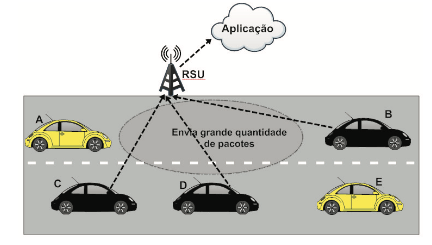
\includegraphics [width=12cm] {images/ataqueddos.png}
	\caption{Ataque DDOS \cite{wanghamsegurancca}.}
	\label{fig:ataqueddos}
\end{figure}
	
	\item {\textbf{Supressão de mensagem}: o atacante recebe e não repassa pacotes da rede com objetivo de impedir que veículos seguintes possam saber de alguma ocorrência, pro exemplo, um aviso de congestionamento, acidentes \cite{tangade2013survey}.}		

	\item {\textbf{Buraco Negro (black hole)}: é uma área onde o tráfego de rede é redirecionado, contudo, ou não há veículos neste local ou nós maliciósos que estão nesta área se recusam a participar, fazendo com que os pacotes da rede não se propaguem. A figura \ref{fig:ataguerubronegro} ilustra o ataque onde veículos se recusam a transmitir a mensagem recebida pelo veículo C.}		
	
\begin{figure}[!h]
	\centering
	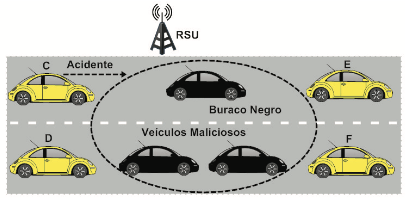
\includegraphics [width=12cm] {images/ataqueburaconegro.png}
	\caption{Ataque Buraco Negro \cite{wanghamsegurancca}.}
	\label{fig:ataguerubronegro}
\end{figure}
	
	\item {\textbf{Jamming}: é um ataque de negação de serviço através do meio físico, onde o ataquente transmite um sinal para pertubar o canal de comunicação o que reduz a relação sinal ruído SNR (Signal to Noise Ratio) para o receptor. Segundo  \citeonline{avelar2015interoperability}, o impacto com esse tipo de ataque é devastador. }			
\end{itemize}

\subsection{Ataques contra a Autenticidade e a Identificação}

\begin{itemize}
	\item {\textbf{Falsificação de endereço (\textit{address spoofing})}: o atacante cria um endereço falso de origem, fazendo com que o nó atacado confie no remetente achando que o mesmo possui permissão para conectar-se à rede \cite{al2012survey}.}
	
	\item {\textbf{Mascaramento}: ocorre quando um veículo malicioso falsifica sua identidade  para se passar por outro com intuito de ter acesso a recursos restritos. Por exemplo, se passar por uma ambulância e ter vantagem no trânsito.}
	
	\item {\textbf{Replicação do certificdo ou chave}: consiste em utilizar certificados ou chaves duplicados, que são usados como prova de identificação com objetivo de criar ambiguidade dificultando assim, a identificação de um veículo pelas autoridades \cite{mejri2014survey}.}
	
	\item {\textbf{Sybil}: é gerado múltiplias identidades por um atacante, para simular vários veículos e cada nó transmite mensagens com múltiplias identidades e assim sucessivamente. Desta maneira, um único veículo pode parecer centenas fazendo que com veículos reais mudem a rota achando que ali há um congestionamento \cite{tangade2013survey}.}
\end{itemize}

\subsection{Ataques contra a Integridade e Confiança dos Dados}

\begin{itemize}
	\item {\textbf{Falsificação nos dados de GPS (\textit{GPS spoofing})}: o atacante utiliza simulador de satélite GPS para gerar sinais  mais fortes que o sinal originado de um satélite real de maneira a enganar os sensores de GPS introduzindo um alocalização falsa \cite{rawat2012vanet}.}
	
	\item {\textbf{Ilusão (ataque contra os sensores do veículo)}: \citeonline{isaac2010security} e \citeonline{al2012survey} disseram que esse e um novo tipo de ameaça em aplicações VANET onde o atacante interfere intencionalmente  nos sensores do seu próprio veículo gerando valores errados com objetivo de criar mensagens de aviso de tráfego incorretas na rede, assim, é criado uma condição de ilusão em VANET. Os métodos tradicionais de autenticação e integridade utilizados em redes sem fio são inadequados contra este tipo de ataque.}
	
	\item {\textbf{Injeção de informação falsa (\textit{bogus information})}: neste tipo de ataque o atacante pode ser um usuário real ou um intruso que transmite informações falsas na rede para obter vantagens  ou afetar decisão de outros veículos. Pode ser chamado de também de ataque social, onde o atacante  procura confundir e distrair a vítima  com envio de mensagens antiéticas para o motorista ficar confuso e distraído podendo causar um acidente como mostra a figura  \ref{fig:ataquesocial}.	}
	
\begin{figure}[!h]
	\centering
	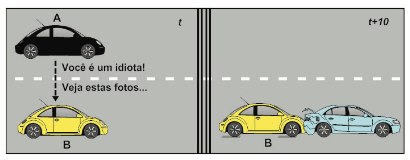
\includegraphics [width=12cm] {images/ataquesocial.png}
	\caption{Ataque social \cite{wanghamsegurancca}.}
	\label{fig:ataquesocial}
\end{figure}	

	\item {\textbf{Modificação de mensagem (\textit{man in the middle})}: de acordo com \citeonline{mejri2014survey}, este ataque a autenticidade do remetente e a integridade das mensagens onde o veículo atacante fica inserido entre dois veículos reais que se comunicam então, o atacante faz o intermédio entre a comunicação interceptando as mensagens enquanto estes acreditam estarem se comunicando diretamente.  A figura \ref{fig:ataquemiddle}  mostra o veículo malicioso M escutado a comunicação entre os veículos A e B, modifica um alerta recebido e propaga uma informação falsa, para os veíulos B e C ) 	}

\begin{figure}[!h]
	\centering
	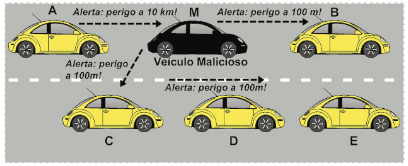
\includegraphics [width=12cm] {images/ataquemainmiddle.png}
	\caption{Ataque demodificação de mensagem \cite{wanghamsegurancca}.}
	\label{fig:ataquemiddle}
\end{figure}

\end{itemize}

\subsection{Ataques contra a Confidencialidade}

\begin{itemize}

	\item {\textbf{Análise de tráfego}: segundo \citeonline{isaac2010security}. esse é um ataque passivo utilizado em redes \textit{ad-hoc}, onde o atacante que tenha acesso à rede pode interceptar o tráfego de pacotes coletando dados que estejam sendo transmitidos sem o uso de criptografia.}

	\item {\textbf{Força bruta}: tem como foco capturar mensagens trocadas  ou ainda o processo de identificação e autenticação. Esse ataque não é trivial já que o tempo de comunicação entre os veículos é relativamente curto e esse ataque consome muito tempo \cite{pathre2013identification}.}

	\item {\textbf{Revelação de identidade}: normalmente, o motorista é o dono do veículo, então, o atacante pode obter a identidade do proprietário de um veículo violando sua privacidade \cite{tangade2013survey} e utilizá-lo para compor informações para um ataque social.}
	
\end{itemize}

\subsection{Outros Ataques}

\begin{itemize}
	
	\item {\textbf{Ataques contra não repúdio (\textit{accountability})}: consiste em tomar medidas para permitir ao atacante negar a realização de uma ou mais ação \cite{wanghamsegurancca}. Apesar disso, \citeonline{mejri2014survey}, não foi encontrando na literatutura um documento afirmando a possibilidade desse ataque.}
	
	\item {\textbf{Ataques contra a privacidade}: estes tidos de ataques violam a privacidade dos usuários e condutores em redes veiculares. Segundo \citeonline{wanghamsegurancca}}, estudos na literaturam classificam esses tipos de ataques como uma categoria separada para VANETs e cita dois exemplos: rastreamento de veículo durante sua viagem e engenharia social, verificando se o veículos encontra-se em deslocamento ou parado \cite{mejri2014survey}.
	
	\item {\textbf{Conluio}: é o ataque que se utiliza de vários nós da rede com um objetivo comum, de realizar o vandalismo ou terrorismo, tendo como resultado a indisponibilidade da rede  ou de algum serviço ou denegrir a reputação de confiança de um veículo \cite{zhang2011survey}.}
	
\end{itemize}

As aplicações suportadas por VANETs com foco em segurança, permite a toamda de decisão por um condutor com base em informações enviadas por outros veículos. Entretanto, se um veículo malicioso cria ou altera mensagens, este pode colocar o motorista em situação de risco \cite{wasef2010complementing}. Dessa forma, a autenticidade das mensagens é fundamental para segurança das redes veiculares e dependendo da aplicabilidade, é necessário ainda fazer uso da criptografia \cite{wanghamsegurancca}. Pensando nisso, vários autores \cite{raya2006securing} \cite{mejri2014survey} escolheram a assinatura digital como solução para autenticação das mensagens contidas nas redes veiculares. 

O método mais simples e eficiente para assinatura digital, é atribuir, a cada veículo, um par chaves possibilitando assinar digitalmente as mensagens. Assim, é necessário utilizar uma autoridade cetificadora confiável implicando no uso de uma Infraestrutura  de Chaves Públicas (ICP) veicular \cite{wasef2010complementing}.

\section{Algoritmos de Roteamento}

Os algoritmos de roteamento em redes veiculares é um dos desafios estabelecidos, já que não existe rotas pré-definidas e nem estimativos da quantidade de nós de uma rede e o fator primordial que é a alta mobilidade dos nós. Então, como calcular as rotas necessárias para encaminhar os pacotes com sucesso, desde a origem até ao destino? 

Foram realizados diversos estudos com a finalidade de comparar o desempenho dos algoritmos aplicados para redes móveis, de modo a corrigir as suas limitações, alguns sofreram adaptações, enquanto outros foram criados \cite{luis2009melhoria}.

Dentre os principais algotirmos de roteamento, com foco nas redes veiculares, temos os protocolos: ad-hoc, baseados em localização, baseado em \textit{clusters}, por \textit{broadcast} e geocast
%Ad-hoc, PRAODV/PROADV-M, GPSR, GSR, A-STAR, COIN, CBLR, Geocast, DRG/ROVER.

\subsection{Protocolos Ad-hoc}

As redes ad-hoc é caracterizada por ser um tipo de rede que não utiliza infra-estruturas e permite a mobilidade dos nós. Ao contrário dos outros protocolos de roteamento infra-estruturados, os quais não apresentam um  desempenho aceitável para redes VANETs.  

São tradicionalmente divididos em duas grandes categorias: reativos e pró-ativos. Os Reativos caracterizam-se pelo fato de nem sempre possuirem as rotas para todos os nós da rede. Quando um nó precisa de uma rota para um certo destino na rede, inicia o processo de descoberta de rota e é finalizado quando a rota e calculada com êxito ou não exista uma rota disponível. As rotas já decobertas são utilizadas enquanto o nó de destino permanecer alcancável ou não ser mais necessário. Os protocolos reativos mais conhecidos são AODV (\textit{Ad hoc On Demand Distance Vector}) e o DSR (\textit{Dynamic Source Routing}). Em contra partida, \citeonline{boukerche2004performance}, afirmou que o desempenho dos protocolos AODV e DSR é bastante prejudicado pela constante alteração topológica da rede.

Os protocolos pro-ativos (\textit{table-driven}) caracterizam-se por ter conhecimento das rotas para todos os nós existentes. Esse protocolo possui a vantagem de ter um reduzido atraso incial, pois as rotas já estão estabelecidas. Não obstante, a metodologia dos protocolos pró-ativos implica na existência de um tráfego adicional para controle da topologia, uma vez que é preciso manter as rotas existentes sempre atualizadas, consumindo uma maior largura de banda. São exemplos de protocolos pró-ativos: DSDV ('\textit{Destination Sequenced Distance Vector}) e o WRP (Wireless Routing Protocol).

Os protocolos PRAODV (\textit{PReemptive AODV}) e PRAODV-M (\textit{PReemptive AODV - Maximum}) foram criados em cima do protocolo AODV, oferecendo uma componente baseado na velocidade, na localização  e na predição. A difererença é que no PRAODV, é estabelecida uma ligação alternativa entre dois nós, antes da principal expirar, e a PRAODV-M, escolhe uma rota que prevê ficar ativa por mais tempo, ao contrário da AODV, que escolhe a rota mais curta \cite{luis2009melhoria}. 

O protocolo OLSR (Optimzed Link State Routing), realiza uma otmização da topologia, sendo este, o algoritmo mais utilizado em redes ad-hoc \cite{jacquet2001optimized}. Possui um modo de funcionamento bastante característico, pois cada nó, seleciona dentre seus vizinhos, uma quantidade de nós suficientes de maneira a cobrir toda a vizinhança a dois saltos do nó, com objetivo de realizar o roteamento e retransmitir as mensagens. 

\subsection{Protocolos Baseados em Localização}

Um dos primeiros protocolos baseados em localização foi o GPSR (Greedy Perimeter Stateless Routing), no qual baseia-se na informação geográfica em relação aos vizinhos. A vantagem deste protocolo está em manter a informação apenas sobre a topologia local, permitindo uma maior escalabilidade e um menor tempo para criação de novas rotas. Entretanto, o desempenho do GPSR é comprometido em ambiente reais, apresentando obstáculos e distribuição aleatória dos veículos.

O protocolo GSR (\textit{Global State Routing}) foi criado com objetivo de corrigir a limitação do GPSR de modo a utilizar o \textit{link-state} de forma que cada nó mantém uma tabela de conectividade, contendo todas as ligações existentes entre os diversos nós da rede, otimizando as decisões a nível de roteamento local. Avaliação feita por  \citeonline{fussler2003mobicom}, indica que o GSR apresentou melhor desempenho em relação ao GPSR e melhora no atraso comparado ao DSR, do mesmo modo que, uma melhor taxa de sucesso de entrega e menor ocupação da largura de banda se comparado com o AODV \cite{li2007routing}.  

O protocolo A-STAR é baseado no GSP e GPSR e incorpora um sistema de sensibilização de tráfego (\textit{traffic awareness}) fazendo uso de mapas das estradas ordenados por utilização, de forma a poder definir suas rotas pelas estradas com maior conectividade, na tentativa de aumentar a probabilidade de sucesso na entrega dos pacotes. Devido à sensibilizaçãode tráfego aplicado ao A-STAR, há um melhor desempenho, entorno de 40\%, na entrega de pacotes em relação ao protocolo GSR.

Foi proposto por  \citeonline{leontiadis2007geopps}, o protocolo de roteamento denominado GeOpps (\textit{Geographical Opportunistic routing for vehicular networks}), ele assume que todos os nós estão munidos com sistemas de posicionamento de maneira a encaminhar um pacote para um nó que está, teoricamente, em melhores condições de poder entregar  ao seu destino final. Segundo  \citeonline{karp2000gpsr}, os resultados mostraram que o protocolo GeOpps tem um melhor comportamento do que o GPSR.

\subsection{Protocolos Baseado em \textit{Clusters} }

Os protocolos de roteamento baseados em \textit{Clusters}, representam uma rede virtual criada por meio de nós de uma rede física, onde o grupo criado. por um conjunto de nós interligados de maneira lógica, tem tendêcia a alterar rapidamente a sua composição.

Cada \textit{cluster} pode apresentar um nó como lider, denomicado \textit{cluster-head}, que é incubido de pela coordenação da comunicação dos nós da rede. Os nós de um cluster podem se comunicar diretamente porém, a comunicação extra grupo deve ser feita somente pelo lider. A criação dos \textit{clusters} é de suma importância para aumentar a escalabilidade dos protocolos de roteamento e está na estabilidade a chave para o desempenho destes algoritmos \cite{luis2009melhoria}.

Em redes veiculares, a aleatoriedade da movimentação dos veículos torna os protocolos de roteamento baseado em cluster para redes móveis frustrados tais como: \textit{Adaptative Clustering} e o MCDS \textit{Minimum Connected Dominating Set} \cite{das1997routing}.

Como dito anteriormente, o sucesso de um cluster está na estabilidade consequentemente, muitas pesquisas foram realizadas com objetivo de tornar o grupo o mais estável possível a exemplo do protocolo COIN \textit{Clustering for Open  IVC Networks} que utiliza informações sobre mobilidade para para formação do \textit{cluster}. Entretanto, são adicionados ao algoritmo as intenções do motorista do veículo como também a dinâmica veicular. De acordo com  \citeonline{blum2003mobility}, resultados demonstram que as otimizações feitas molhoram o desempenho do protocolo, identificando um aumento de 192\% no tempo  médio de vida de um \textit{cluster} e uma redução de 42\% no número de alterações dos integrantes do grupo.

O protocolo CBLR (\textit{Cluster-Based Location Routing algorithm}) apresentado por  \citeonline{santos2004cluster}, utiliza conceitos de \textit{cluster} juntamente com informações de localização. Este protocolo, se comparado ao AODV e DSR, desmostrou um desempenho superio ao atraso \textit{end-to-end} e à taxa de sucesso de entrega.


\subsection{Protocolos  por Broadcast}

Os protocolos de roteamento baseados em broadcast, consistem em transmitir informações por todos os nós que façam parte da rede. Em VANETs, este tipo de defusão é muito utilizado para compartilhar informações sobre o tráfego, condições da estrada, condição do clima, entre outros \cite{luis2009melhoria}. Assim,  fica garantido que todos receberam a informação. Entretanto, o funcionamento destes protocolos não é indicado para redes consideravelmente grandes, podendo gerar um efeito de tempestade de broadcast (broadcast storm), aumentando a probalilidade de colições de pacotes e o consumo da largura de banda, comprometendo o desempenho.

O protocolo BROADCOMM (\textit{BROADcast COMMunications}) apresenta algumas semelhanças com os protocolos baseados em clusters ao dividir a auto-estrada em células e utilizar o conceito de \textit{cluster-head}, aqui chamando de \textit{cell-reflectors} \cite{durresi2005emergency}. Neste caso, a diferença é que as \textit{cell-reflectors} devem ficar geometricamente no centro da célula. A função do \textit{cell-reflectors} é difundir as informações de emergências entre as células. Contudo, este protocolo funciona apenas para ambiente de auto-estrada.  

\subsection{Protocolos \textit{Geocast}}

O protocolo de \textit{Geocast} (\textit{Geocast Routing}) leva em consideração a posição/localização, e seu objetivo é entregar um pacote a nós que estão em uma determinada região denominada ZOR (\textit{Zone of Relevance}). A implementação deste protocolo deve levar em consideração, a integração de um serviço de multidifusão em conjunto com o agrupamento dos nós confome seu posicionamento geográfico, criando assim as ZORs.

Uma implementacão do algoritmo \textit{Geocast} foi utilizado na construção do protocolo \textit{Message Dissermination Process} proposto por  \citeonline{briesemeister2000disseminating}, cuja objetivo é evita colisão de pacotes e diminuir o número de retramissões. No momento que um nó recebe um pacote, ele não o encaminha imediatamente esperando um tempo de  modo a poder tomar uma decisão referente à retransmissão. O tempo de espera é baseado na distância do nó que lhe enviou o pacote, ou seja, quanto maior a distância menor é o tempo de espera. Quando o perído de tempo expira, o pacote somente e retransmitido se a informação não tiver sido recebida novamente. Esse controle no envio dos pacotes  faz com que seja menos provável a existêcia de \textit{broadcast stoms} e a propagação de pacotes seja mais eficiente.

Os protocolos DRG (\textit{Distributed Robust Geocast}) e ROVER (\textit{RObust Vehicular Routing}) projetados por \citeonline{kihl2008design}, sendo o DRG um protocolo com foco em grandes cenários, adaptável às constantes mudanças da topologia das redes veiculares e fornece um sistema de encaminhamento rápido e confiável. Em contra partida, o protocolo ROVER oferece uma difusão \textit{multicast} confiável, tendo como base, um processo de descoberta de rotas dentro da ZOR.

\subsection{Comparação dos Protocolos de Roteamentos}

Ainda não foi encontrada a melhor forma de se criar um protocolo de roteamento para VANETs, porém, há autores que consideram um roteamento baseado em cluster mais viável em relação aos outros modelos \cite{luis2009melhoria}. A aplicabilidade do protocolo faz aumentar o número de pesquisas existentes sendo que, se há alguns protocolos que possuem desempenho favorável em cenários urbanos, isso já não acontece em ambientes de alta mobilidade, e vice-versa. A tabela \ref{tab:roteamento} faz um apanhado geral sobre os protocolos de roteamento e os cenários mais indicados.

\begin{longtable}{ p{.15\textwidth}  p{.13\textwidth}   p{.22\textwidth}  p{.15\textwidth} p{.17\textwidth}} 
	\hline
	\rowcolor[gray]{0.7}
	Protocolo de Roteamento	& Tipo Protocolo & Informação Sobre Posição  & Estrutura Hierárquica & Cenário de Mobilidade  \\ \hline
	
	AODV	& Unicast & Não & Não & ---  \\ \hline
	DSR	& Unicast & Não & Não & ---  \\ \hline
	OLSR	& Unicast & Não & Não & ---  \\ \hline
	PRAODV-M	& Unicast & Seleção de rotas & Não & Auto-estrada  \\ \hline
	GPSR	& Unicast & Encaminhamento de Pacotes & Não & ---  \\ \hline
	GSR	& Unicast & Encaminhamento de Pacotes & Não & Urbano  \\ \hline
	A-STAR	& Unicast & Encaminhamento de Pacotes  & Não & Urbano \\ \hline
	GeOpps	& Unicast & Encaminhamento de Pacotes & Não & Urbano  \\ \hline
	COIN	& Unicast & Formação de Cluster & Sim & Auto-estrada  \\ \hline
	CBLR	& Unicast & Encaminhamento de Pacotes & Sim & Circuito circular e quadrangular  \\ \hline
	%Flooding	& Broadcast & Não & Não & ---  \\ \hline
	BROADCOMM	& Broadcast & Formação de células & Sim & Auto-estrada  \\ \hline
	Msg. Diss. Proc.	& Geocast & Encaminhamento de Pacotes & Não & Auto-estrada  \\ \hline
	DRG	& Geocast & Encaminhamento de Pacotes  & Não & Auto-estrada  \\ \hline
	ROVER	& Geocast & Encaminhamento de Pacotes  & Sim & Auto-estrada  \\ \hline
		
	\caption{Protoclos de roteamento aplicados a redes veiculares \cite{luis2009melhoria} } % needs to go inside longtable environment
	\label{tab:roteamento}
\end{longtable}

\section{Aplicações}

Há uma série de aplicações que as redes veiculares podem atuar porém, para cada aplicação é necessário conhecer as caracteristicas que as cercam, tais como: segurança da informação; tempo de resposta; garantia na entrega; entre outros.

Segundo \citeonline{autoentusiastasclassic}, há uma relação entre velocidade dos veículos e a distância entre eles, esta relação é diretamente proporcional indicando que quanto maior a velocidade, maior deve ser a distância entre os veículos. Isto ocorre naturalmente, pois o motorista precisa considerar-se seguro no trânsito. Porém, esta condição é dinâmica variando a cada instante, e para agravar, a relação entre velocidade do fluxo e a distância dos veículos relaciona um fator de realimentação positiva, e sistemas com esta característica, tendem à instabilidade, gerando transtornos no trânsito. Então, um sistema capaz de alertar o motorista caso o mesmo esteja a distância ``não segura'' do veículo da frente, pode ser alcançado com sistemas baseados em VANETs. 

Outra aplicação, com foco em redes veiculares, pode ser produdizida por meio de alertas de colisão em uma via de fluxo intenso, o condutor possui um tempo de percepção mais um tempo de reação e somente após a soma dos tempos, poderá executar uma reação. Esta situação mostra a importância de agregar aos veículos uma rede de comunicação no qual os mesmos e seus motoristas, poderão trocar informações de ocorrências emergenciais e preventivas no trânsito. Esta situação fica claramente evidenciada na figura \ref{fig:vanetqian}. 

\begin{figure}[!h]
	\centering
	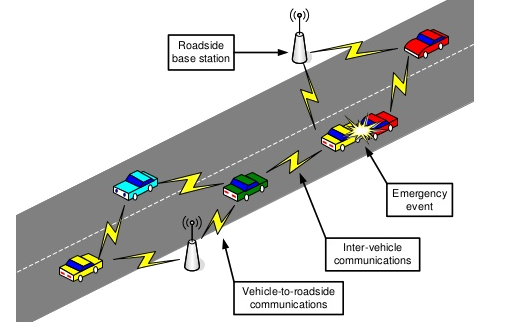
\includegraphics [width=12cm,height=7cm] {images/vanet_qian.png}
	\caption{Exemplo de aplicação VANET \cite{qian2008secure}.}
	\label{fig:vanetqian}
\end{figure}

Há também a possíbilidade de aplicações voltadas para o entretenimento com o uso de \textit{chats} ou até mesmo propagandas comerciais nas proximidades do veiculos.

Por ser uma área crescente, as redes veiculares tem atraído empresas automobilisticas e órgãos controladores  a exemplo do órgão americano de pesquisa de inovação tecnológica, RITA (\textit{Research and Innovative Technology Administration}) o qua é coordenado pelo departamento de transporte dos EUA. O projeto Car 2 Car (\textit{Communication Consortion}), criado por cinco fabricantes de automóveis europeus (BMW, Volvo, Volkswagen, Honda, e Audi) e apoiada por fornecedores de equipamentos, organizações de pesquisa e outros parceiros, tendo como objetivo  aumentar ainda mais a segurança e a eficiência do tráfego rodoviário através de Sistemas de Transporte Inteligente (C-ITS) cooperativos com a comunicação veículo para veículo (V2V) suportada pela comunicação veículo infraestrutura (V2I) . 

\chapter{Arquitetura I9Vanet}\label{sec:i9vanet}

\section{Visão Geral}
A arquitetura proposta tem a finalidade de criar redes veiculares virtuais em nuvem com foco no auxílio dos principais desafios relacionados à VANETs tais como: alta densidade, baixa densidade, alta mobilidade, segurança e privacidade, entre outros. 

A arquitetura consiste em um modelo aberto, dividido em módulos com funções bem definidas. Cada módulo possui funcionalidades específicas e padrões de comportamentos. Sendo possível estender suas operações ou até mesmo substituí-las de maneira que atenda às novas necessidades.

\section{Módulo da Arquitetura I9Vanets}

A Figura \ref{fig:dModulos} mostra os módulos necessários da arquitetura I9VANETS:  \textit{Applications, Server Management Cloud, Routing between Nodes, Secutity OBU/RSU, Infra-Cloud Communication} e \textit{Vehicle-Cloud Communication}. Sendo que cada módulo segue um modelo de arquitetura com objetivos bem definidos, sendo que suas interfaces de comunicação são padronizadas, permitindo substituir um módulo por outro, com a mesma característica, sem que interfira no modelo.

\begin{figure}[!h]
	\centering
	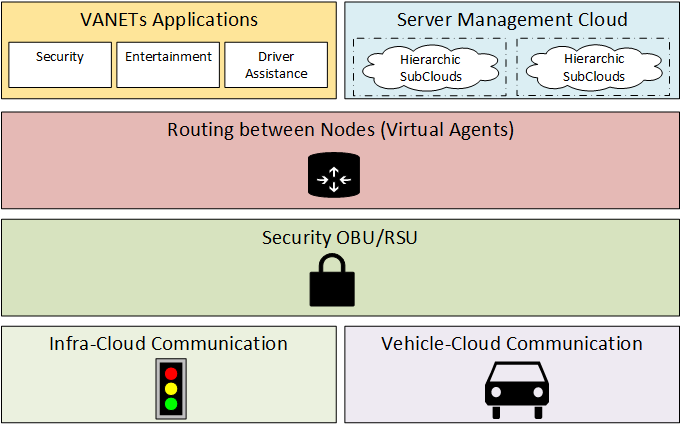
\includegraphics [width=12cm,height=7cm] {images/modulos.png}
	\caption{Módulos definidos para a arquitetura I9Vanet.}
	\label{fig:dModulos}
\end{figure}

Todas as classes que podem ser customizadas tais como: a tecnologia de comunicação; algoritmo de roteamento; modelo de segurança; implementação de eventos, devem estar definidas no arquivo de configuração \textbf{idclassload.properties} como os ítens abaixo.

\begin{itemize}
	\item{\textbf{ICommunication}:
		
		 br.com.virtualVanets.infraVehicle.communication.CommunicationWebSocketImpl}	

	\item{\textbf{CommunicationV2A}:
		
		br.com.virtualVanets.infracloud.communication.impl.CommunicationI2AImpl}	
	\item{\textbf{CommunicationI2A}:
		
		br.com.virtualVanets.infracloud.communication.impl.CommunicationI2AImpl}	
	\item{\textbf{ListenerInfraEquipament}:
		
		br.com.virtualVanets.applicationModel.listener.DefaultListenerInfraEquipament}	
	\item{\textbf{ListenerVehicle}:
		
		br.com.virtualVanets.applicationModel.listener.DefaultListenerVehicle}	
	\item{\textbf{EventInfraEquipament}:
		
		br.com.virtualVanets.infracloud.listener.SVVEventInfraEquipament}	
	\item{\textbf{EventVehicle}:
		
		br.com.virtualVanets.vehiclecloud.listener.SVVEventVehicle}	
	\item{\textbf{SecurityModel}:
		
		br.com.virtualVanets.security.I9Security}	
	\item{\textbf{RouterNetwork}:
		
		br.com.virtualVanets.infraVehicle.communication.CommunicationWebSocketImpl}	

\end{itemize} 


\subsection{Módulo de Comunicação}

O módulo de comunicação é responsável por definir o modelo de troca de mensagens entre os servidores e os dispositivos  OBU e RSU. Dessa forma, é possível mudar o protocolo de comunicação sem interferir na arquitetura. 
% **** falar sobre a cumunicação no sentido de ser multicast e como funciona o boreadcast

\subsubsection{Comunicação Infra-Cloud}

A forma como a comunicação será efetivamente implementada, não é preocupação da arquitetura, cabe ao desenvolvedor utilizar a tecnologia (socket, webservices, websocket, push, etc) que mais se adequa à sua necessidade e/ou região. As informações trocadas são de entrada e saída, portanto, os equipamentos RSU podem enviar como também receber informações dos servidores. Em VANETs, pode existir a comunicação entre veículos e dispositivos à beira da rodovia (V2I), todavia, não é o propósito desta arquitetura realizar, de forma direta, a comunicação entre os equipamentos contudo, será realizada entre os respectivos agentes virtuais . 

Todos os equipamentos RSU serão virtualizados e representados por agentes virtuais. Sendo assim, pode haver a comunicação entre agente RSU e o agente do veículo (AV2AI), como também entre agentes RSUs (AI2AI), como mostrado na Figura \ref{fig:dComunicacaoAgentes}.

Os dispositivos RSUs disponibilizam as seguintes informações: identificação, latitude, longitude, altitude, temperatura, pressão, umidade relativa do ar e um campo textual para informações extras. A plataforma prevê  3 operações:

\begin{itemize}
	\item{\textbf{Conectar}: realiza a conexão com o servidor, informando identificador do dispositivo, a latitude e longitude;}	
	\item{\textbf{Enviar Mensagem}: envia mensagens para rede. O conteúdo das mensagens variam de acordo com a aplicação;}	
	\item{\textbf{Disconectar}: fecha a conexão com o servidor.}	
\end{itemize} 

Para implementar a comunicação entre o agente e o veículo (I2AI), é necessário implementar a classe abstrata \textbf{CommunicationI2A} e sobrescrever o método \textbf{sendMsg}. Esse método é executado pela arquitetura de maneira transparente e deve enviar o comando para o dispositivo. 


\subsubsection{Comunicação Veículo-Cloud}

Define a comunicação entre os servidores e os equipamentos instalados nos veículos (OBU). Os detalhes da implementação podem ser substituídos permitindo utilizar a melhor tecnologia do momento. Assim como no módulo de Comunicação Infra-Cloud, a comunicação V2V não ocorrerá diretamente, como ocorre nos modelos tradicionais, ela será rea;zoada através dos agentes virtuais, que nada mais são do que a representação virtual dos veículos. Desta forma, a comunicação se dará entre os agentes (AV2AV) e entre o agente e o veículo físico (V2A) este processo é exemplificado na Figura \ref{fig:dComunicacaoAgentes}.
  
\begin{figure}[!h]
	\centering
	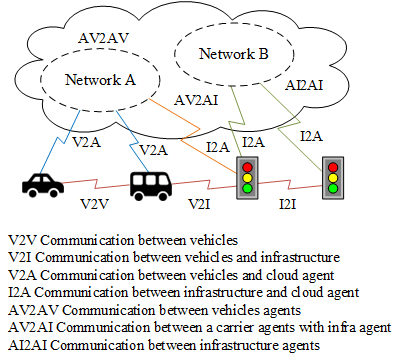
\includegraphics [width=12cm,height=8cm] {images/agentemoveis_virtuais.png}
	\caption{Modelo de comunicação V2A, I2A, AI2AI e AV2AI.}
	\label{fig:dComunicacaoAgentes}
\end{figure}

O veículo deve disponibilizar as seguintes informações: identificação, latitude, longitude, altitude, velocidade, direção, tipo operação e um campo textual. A plataforma prevê 4 operações que podem ser extendidas, são elas:

\begin{itemize}
	\item{\textbf{Conectar} (CONNECT\_CODE): realiza a conexão com o servidor, informando identificador do dispositivo, a latitude e longitude;}	
	\item{\textbf{Movimentar} (MOVIMENTATION\_CODE): este comando é executado a cada 10 segundos, com o intuito de informar a geolocalização, velocidade e direção do mesmo;}	
	\item{\textbf{Enviar Mensagem} (SEND\_BROADCAST\_CODE): envia mensagens para os veículos da rede, sendo que o conteúdo das informações variam de acordo com a aplicação;}	
	\item{\textbf{Disconectar} (DISCONNECT\_CODE): fecha a conexão com o servidor removendo-o da rede.}	
\end{itemize} 

Para implementar a comunicação entre o agente e o veículo (V2AV), é necessário implementar a classe abstrata \textbf{CommunicationV2A} e sobrescrever o método \textbf{sendMsg}. Este método é responsável por chamar a classe responsável pela conexão efetivamente definida.


\subsection{Módulo de Segurança}

%Responsável pela segurança e privacidade dos equipamentos instalados nos veículos (OBU) e nas rodovias (RSU). Exatamente como os módulos de comunicação, este pode ser substituído por novas implementações. O objetivo é garantir que os equipamentos vinculados aos agentes virtuais sejam legítimos, não permitindo fakes (agentes maliciosos que ocultem a sua identidade). Para isso, foi desenvolvido a segurança baseada no método assincrono para assinatura e criptografia da mensagem.

A segurança na troca de informações em redes veiculares é um dos desafios que devem ser solucionado antes mesmo da implantação de uma solução VANET ser posta no mercado, então, como garantir os princípios da autenticidade, integridade, confidencialidade e  não repúdio na troca de mensagens entre os veículos? Já que é inviável fornecer as chaves de segurança de todos os veículos durante a comunicação. 

Na arquitetura I9Vanet, foi pensado em um processo de comunicação entre os equipamentos, OBU e RSU, e os servidores em Nuvem, de forma que deva garantir os princípios da autenticidade, integridade, confidencialidade e não repúdio através do uso de assinatura digital baseado em algoritmos assimétricos e criptografia dos dados toda via, este último foi defiinido de forma parametrizada para que fosse feito análise comparativo entre a comunicação aberta e criptografada.

A geração das chaves para cada equipamento deve ser controlado pelo órgão responsável pelos veículos, a exemplo, o DENATRAN (Departamento Nacional de Trânsito). Quando um novo veículo for cadastrado em sua base, ``veículo zero quilômetro'', deve ser gerado as chave pública e privada, sendo que a pública deva ser enviada para os servidores em nuvem  responsáveis  pelo gerenciamento da arquitetura I9Vanets e a privada, inserida no equipamento.

A cada renovação de licenciamento, um novo token deve ser gerado e forneceido ao equipamento e publicado nos servidores. Como também, em caso de venda de um veículo, ao passar para o nome do novo proprietário, deve ser gerado um novo token.

Se o parametro de criptografia estiver habilitado, o primeiro passo no momento da conexão é a troca de chave secreta para que toda comunicação seja segura. Para isso, assim que o comando \textit{onConnection} for executado, o servidor enviará o comando \textit{createSecretKey} com a chave secreta criptografada com a chave pública do veículo assim, o mesmo poderá descriptografar com sua chave privada e utilizá-la na criptografia de cada mensagem de agora em diante. 

No momento que um equipamento desejar enviar uma mensagem para seu agente em nuvem, ela deve ser asinada com sua chave privada, assim, através da verificação da assinatura com a chave pública, o agente poderá conviar no remetente. Porém, a mensgaem será asisnada com a chave secreta do servidor para que o equipamento, OBU ou RSU, possa validar através da chave pública do servidor.

%Para o momento, não foi necessário criptografar a mensagem, mas este passo pode ser inserido restando apenas avaliar o custo de processamento tanto nos servidores quanto nos dispositivos OBU e RSU.

Alterar o modelo de segurança adicionando novas regras, é possível através da implementação da classe \textbf{ASecurityModel} e dos métodos \textbf{verifySign, sign, encrypt e decrypt}. A chamada dos métodos é feita pela arquitetura de maneira transparente, não sendo necessário intervenção do usuário.

\subsection{Módulo de Gerenciamento dos Servidores}
%Não há limite para o número de servidores na plataforma, a complexidade do ambiente é quem irá determinar o número necessário. Entretanto, eles devem estar organizados de maneira hierárquica, permitindo o gerenciamento de ``sub-clouds'' com objetivo de dividir uma região em localidades menores e poder atender um ambiente maior e mais complexo. Cada servidor deverá ser responsável por uma área mapeada e definida através de cercas virtuais. Quando um nó da rede sair de uma cerca e entrar em outra, a sua representação virtual será transferida para o servidor correspondente a esta nova área.

%Não é possível prever a quantidade de veículos conectatos a um servidor, e isto criou a necessidade de aumentar a capacidade de dispositivos conectados através de uma plataforma de gerenciamento de servidores.

Não é possível prever a quantidade de veículos conectatos a um servidor, e isto criou a necessidade de construir uma plataforma de gerenciamento com objetivo de aumentar a capacidade de dispositivos conectados à arquitetura. Então, pensando nisso, foi definido que os servidores devem ser distribuídos hierarquicamente de forma que permita controlar regiões, denominadas domínio, separadamente e independentemente. Cada servidor deverá conter informações do servidor pai, no caso, o servidor nível 0, o qual  não possui pai. A figura \ref{fig:dDominios} mostra como um exemplo de domínio, onde cada cerca representa um servidor.

\begin{figure}[!h]
	\centering
	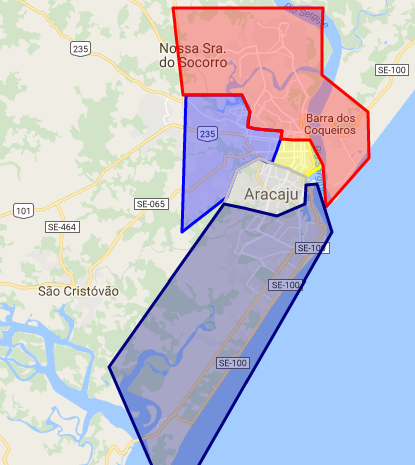
\includegraphics [width=9cm,height=10cm] {images/dominios.png}
	\caption{Exemplo de domínios.}
	\label{fig:dDominios}
\end{figure}


Quando um veículo iniciar a transmissão, será conectado automaticamente ao servidor Nível 0, informando o comando \textit{StartConnection}, o qual realizará uma busca pela coordenada GPS enviada pelo veículo para localizar o servidor responsável pelo domínio onde encontra-se o veículo, podendo ocorrer duas situações:
\begin{enumerate*}
	\item{O veículo apresenta-se em uma área sem cobertura de cerca virtual, assim,  o próprio servidor raiz será responsável por gerenciar a rede VANET deste veículo;}
	\item{O veículo encontra-se em uma domínio válido que é de responsabilidade de algum servidor filho. Então o servidor nível 0 irá passar o comando,  \textit{ChangeServer},  informando o ip do servidor que deve ser responsável pela rede dessa domínio,  e assim o veículo faz uma nova conexão para o novo servidor.}
\end{enumerate*}
 

Cada movimentação do veículo deve ser transmitida para o servidor do domínio, pelo comando \textit{SendMoviment}, o qual verificará se o veículo ainda está em sua região, de acordo com a cerca virtual. Caso não esteja mais sob seu domínio, o servidor irá enviar o comando \textit{ChangeServer} com o endereço do servidor Pai. Assim, o veículo poderá refazer a conexão com este novo servidor, através do comando \textit{StartConnection}, o qual deverá verificar se a coordenada pertence a este servidor ou de algum de seus filhos, este processo é realizado para todos os níveis da hierarquia.

Em todos os servidores deve existir uma base de dados para definir a hierarquia, os domínios geográficos como também o cadastro dos dispositivos. As tabelas \ref{tab:serverTable} e \ref{tab:deviceTable} mostram respectiviamente o dicionário de dados da tabela \textit{server} e \textit{device} utilizadas no sistema.

\begin{longtable}{ p{.20\textwidth}  p{.15\textwidth}   p{.40\textwidth}  p{.20\textwidth}} 
	\hline
	\rowcolor[gray]{0.7}
	Tabela \textit{Server}	& 	&  \\ \hline
	\rowcolor[gray]{0.7}
	Coluna	& Tipo do Dado	& Descrição \\ \
	server\_id	& \textit{integer} & Identificador único no sistema 	\\ \
	address	& \textit{varchar}	& Endereço Ip do servidor \\ \
	server\_idsuper	& \textit{integer} & Identificador do servidor pai 	\\ \	
	dominio	& \textit{polygon} & Cerca virtual de responsabilidade do servidor	\\ \	\\ \hline
	\caption{Colunas das tabelas \textit{Server}. } % needs to go inside longtable environment
	\label{tab:serverTable}
\end{longtable}

\begin{longtable}{ p{.20\textwidth}  p{.15\textwidth}   p{.40\textwidth}  p{.20\textwidth}} 
	\hline
	\rowcolor[gray]{0.7}
	Tabela \textit{Device}	& 	&  \\ \hline
	\rowcolor[gray]{0.7}	
	Coluna	& Tipo do Dado	& Descrição \\ \hline
	device\_id	& \textit{integer} & Identificador único no sistema	\\ \
    identification	& \textit{varchar} & Identificador do dispositivo (Imei, Mac Addess, etc.)	\\ \
    type	& \textit{char} & Tipo do dispositivo (OBU ou RSU)	\\ \
    public\_key	& \textit{byte[]} &  Chave pública do dispositivo	\\ \
		& \textit{integer} & 	\\ \	\\ \hline
	\caption{Colunas da tabela \textit{Device}. } % needs to go inside longtable environment
	\label{tab:deviceTable}
\end{longtable}

A Figura \ref{fig:dServidores} mostra como os servidores devem ser organizados para melhor controle. O servidor nível 0 é a raiz da árvore e responsável por gerenciar os nós abaixo dele. A estrutura não é um uma árvore binária e sim uma formação em árvore com N nós filhos. Quando um veículo que está conectado a um servidor precisar conectar-se a outro, a mudança deve ser solicitada ao servidor pai imediato, caso este não seja o de destino, deve perguntar ao pai deste e assim sucessivamente até encontrar o servidor responsável pelo domínio de destino ou o servidor nivel 0 será responsável por este gerenciamento.
.
\begin{figure}[!h]
	\centering
	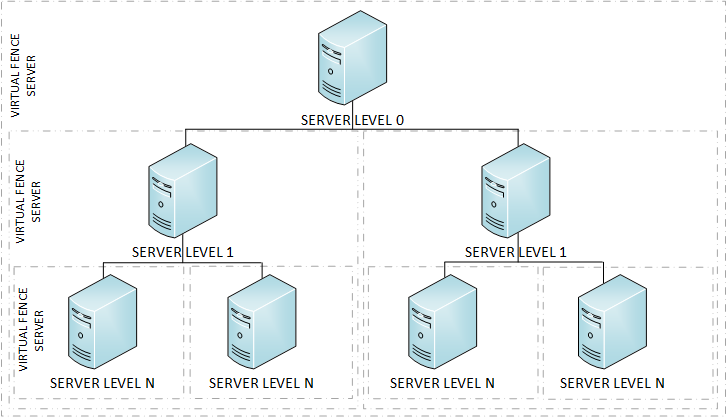
\includegraphics [width=12cm,height=7cm] {images/servidores.png}
	\caption{Organização dos servidores na nuvem.}
	\label{fig:dServidores}
\end{figure}

A cada envio do comando \textit{SendMoviment} pelos veículos, o servidor deve verificar se o mesmo ainda encontra-se no mesmo domínio, como este processo é executado a cada 10 segundos por cada veículo, foi necessário realizar essa consulta em memória ao invés de ir no banco. Para isso, foi utilizado a API GEOTools.

O GeoTools é uma biblioteca feita em Java \textit{open source} que provê ferramentas para manipulação de dados geoespacial em memória. O objetivo da biblioteca é permitir que programadores que estejam desenvolvendo aplicações geoespaciais se concentrem na construção do negócio fim, enquanto reutilizam ferramentas genéricas para funções básicas \cite{hall2008open}.

A mesma funcionalidade do GeoTools poderia ser atingida com o as funções do Postgis porém, ao realizar pequenos testes, foi percebido que o tempo da consulta é 10 vezes maior que a do GeoTools, o que poderia comprometer a avaliação da arquitetura.


\subsection{Módulo de Roteamento}

O módulo de roteamento em ma rede veícular é um dos grandes desafios e por isto, é foco de estudos na busca de soluções que viabilizem a rede. Na arquitetura I9Vanet proposta, essa preocupação está presente porém, a plataforma permite criar novos algoritmos sem a necessidade de preocupar-se com detalhes como, segurança, protocolo de comunicação ou quantidade de veículos.

Toda comunicação entre os nós é realizado entre os agentes virtuais da rede (AV2AV e AV2AI e AI2AI). As regras de roteamento podem ser substituídas ou expandidas, basta implementar novos algoritmos seguindo o modelo da arquitetura do módulo. Quando houver a necessidade de enviar algo para algum nó físico da rede, esta mensagem deve ser enviada através do Módulo Comunicação Veículo-Cloud ou Infra-Cloud e eles se responsabilizarão pela entrega.

%O módulo e roteamento pode ser definido de acordo com a necessidade, bastando implementar a classe \textbf{RouterNetwork} porém, para fins de avaliação da arquitetura, foi implementado o algoritmo que utiliza os RSU como cluster da rede. Pondendo ser utilizando RSU físicos ou virtuais, ou seja, não é necessário implantar um RSU à beira da rodovia, basta definir pontos no mapa e este pode funcionar como um RSU virtual, tendo o comportamento de cluster da rede VANET.

O módulo e roteamento pode ser definido de acordo com a necessidade, bastando implementar a classe \textbf{RouterNetwork} porém, para fins de avaliação da arquitetura, foi construído o algoritmo conhecido como \textit{geocast routing}, no qual o objetivo é entregar um pacote aos nós que pertencam a uma certa região, denominada \textit{Zone of Relevance} que utiliza um OBU como nó cabeça de uma rede veicular.
% os RSU como cluster da rede. Pondendo ser utilizando RSU físicos ou virtuais, ou seja, não é necessário implantar um RSU à beira da rodovia, basta definir pontos no mapa e este pode funcionar como um RSU virtual, tendo o comportamento de cluster da rede VANET.

Os veículos quando iniciam o processo de conexão com o servidor, buscam uma rede  já existente para se conectar. O veículo ``cabeça'' desta rede, deve estar a uma distância máxima de 1 KM e seguir na mesma direção na via, caso contrário, este veículo criará uma nova rede esperando que novos veículos solicitem acesso.

A cada transmissão de um veículo, através da operação \textbf{MOVIMENTATION\_CODE}, o algoritmo de roteamento seguirá uma dentre três opções, são elas: permanecer na rede atual; entrará em uma nova; criará uma nova rede veicular.


%Os veículos escolhem um RSU para participar da rede e a escolha é feita calculando o RSU mais próximo. Porém, a cada transmissão de uma nova coordenada pelo OBU, não é necessário buscar um novo RSU mais próximo, uma vez que é definido uma distância máxima para que o veículo permaneça na rede de uma RSU, quando essa distância for rompida, ai é realizado novamente o processo de busca de um RSU mais próximo.

**** Adicionar Figuras mostrando as 3 possibilidades da rede

\subsection{Módulo de Aplicações}
Permite adicionar novas aplicações tendo como base os recursos disponibilizados pelos outros módulos. Porém, para que as aplicações possam enviar e receber informações da arquitetura, é necessário definir um contrato com as classes da arquitetura, através do uso de interfaces e classes abstratas. Sendo assim, quando um veículo enviar uma informação para seu agente virtual, a arquitetura irá executar um método padronizado de uma classe da aplicação, fazendo com que os dados sejam entregues corretamente.

Podem ser implementados váriados tipos de aplicações com os dados que a arquitetura já disponibiliza porém, caso seja necessário que uma aplicação possa modificar os dados de entrada e saída da arquiteura, é possível utilizar o campo mensagem para adicionar novas informações e assim atender às novas demandas.

\section{Processo de Negócio}

A figura \ref{fig:bpmcriptografia} e \ref{fig:bpm} mostram os diagramas de processos de negócio da arquitetura I9Vanet com e sem criptografia respectivamente. No primeiro processo, o inicio, figura \ref{fig:bpmcriptografia}(1), se dar quando o veículo é ligado e abre a primeira conexão com o servidor raiz, figura \ref{fig:bpmcriptografia}(2). Em seguida, o processo de negociação da chave a ser utilizada na criptografia figura \ref{fig:bpmcriptografia}(3), a chave é criptografada, pelo servidor com a chave pública do veículo e enviada  para o nó da rede, figura \ref{fig:bpmcriptografia}(4). A partir deste momento, toda comunicação será criptografada e em ambos os modelos, toda mensagem será assinada. 

\begin{figure}[h!]
	\centering
	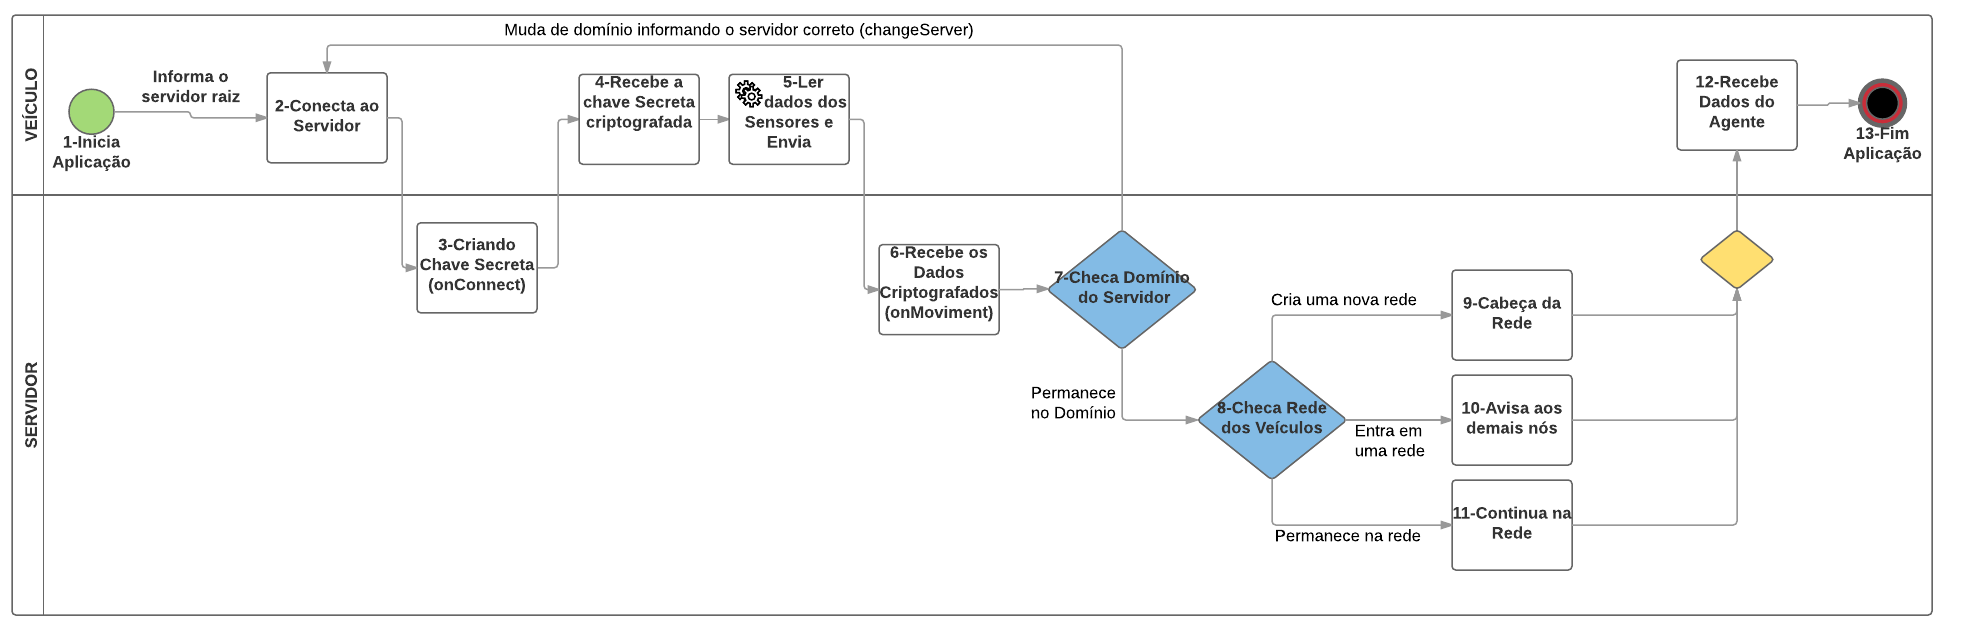
\includegraphics[width=1.0\columnwidth]{images/BPMCriptofrafado.png}
	\caption{Modelo de processo de negócio da arquitetura I9Vanet com criptografia.}
	\label{fig:bpmcriptografia}
\end{figure}

\begin{figure}[h!]
	\centering
	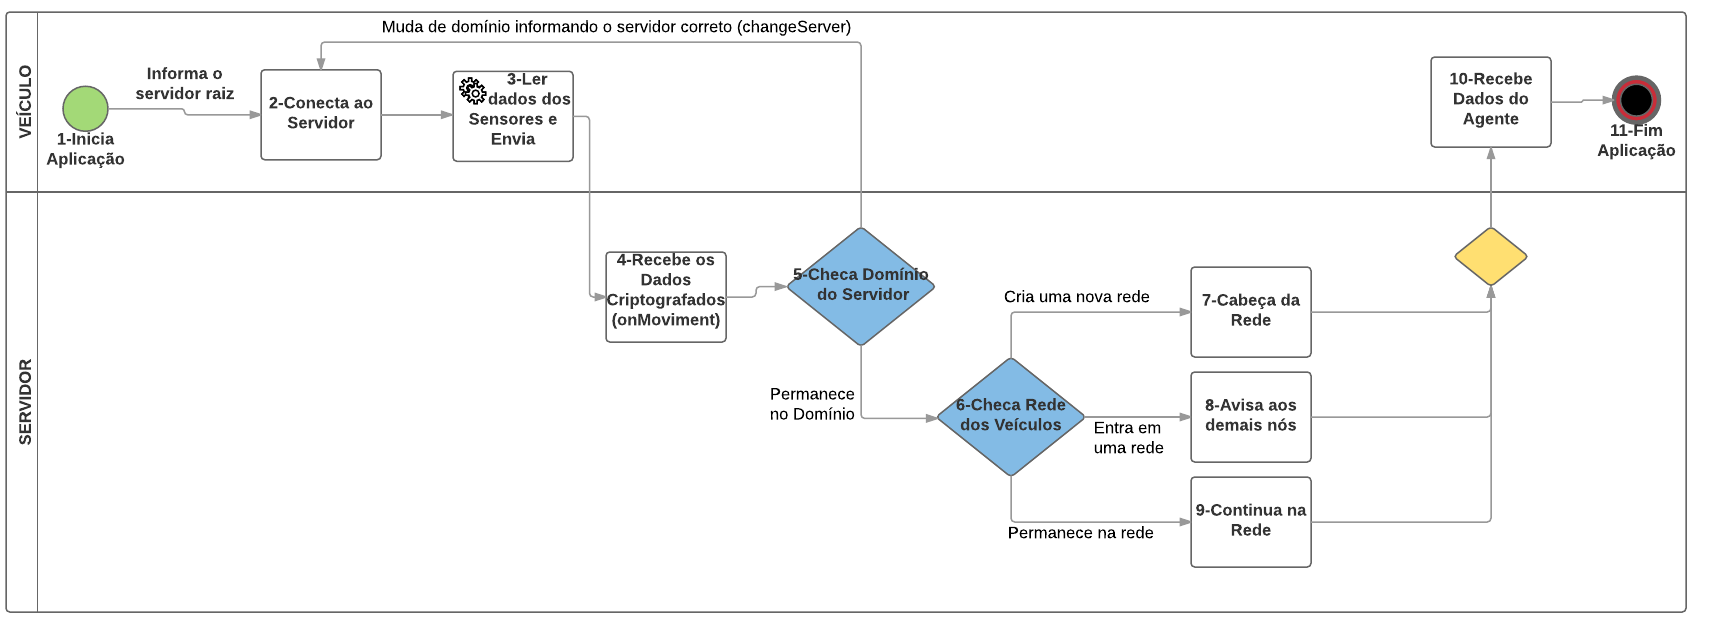
\includegraphics[width=0.9\columnwidth]{images/BPM.png}
	\caption{Modelo de processo de negócio da arquitetura I9Vanet sem criptografia.}
	\label{fig:bpm}
\end{figure}

Após estabelecido o canal seguro, é iniciado uma thread, figura \ref{fig:bpmcriptografia}(5), responsável por obter os dados dos sensores do veículo e enviá-los para o servidor, figura \ref{fig:bpmcriptografia}(6), dentre os dados estão a latitude, longitude, velocidade e direção. O recebimento dos dados é feito pelo método \textbf{onMoviment} que irá verificar o em qual domínio o servidor deve ficar conectado, figura \ref{fig:bpmcriptografia}(7), se a coordenada geográfica indicar que o veículo deve mudar de servidor, então, o comando \textbf{changeServer} é acionado informando o endereço do servidor ``pai'', voltando para o processo, figura \ref{fig:bpmcriptografia}(2), para recriar a conexão e segurança do canal. Caso permaneça no mesmo domínio, deve realizar uma análise sobre a rede que o veículo pertence, verificando se deve permanecer na rede atual, figura  \ref{fig:bpmcriptografia}(11), cria uma  nova rede, figura \ref{fig:bpmcriptografia}(9), ou entrar em uma outra,  \ref{fig:bpmcriptografia}(10).

O processo de execução da rede em si, não está mapeado nesse fluxo de processos já que as mensagens a serem trocada entre os nós da rede, depende da camada da aplicação que está sendo desenvolvida.

\chapter{Avaliação da Arquitetura}\label{sec:avaliacaoArquitetura}

%Com o objetivo de avaliar a plataforma para redes veiculares desenvolvida, chamada de I9Vanet, principalmente no que diz respeito à sua capacidade de comunicação entre nós  da rede, foram realizados alguns experimentos.

Este capítulo visa avaliar a arquitetura I9Vanets,  através do paradigma GQM (Goal-Question-Metric) muito usado para planejar medições em projetos de softwares \cite{van2002goal}. As seguintes fases foram analisadas durante o processo de avaliação: fase de planejamento, de coleta de dados e de interpretação dos resultados.

O processo de avaliação iniciou-se na fase de planejamento com o intuito de analisar a arquitetura com relação à eficácia e eficiência da solução. O experimento teve como público alvo os desenvolvedores de software interessados na arquitetura como gerenciamento de uma rede VANET para ITS no contexto de cidades inteligentes.

Com base na proposta da arquitetura i9Vanets, foram realizados dois tipos de testes. O primeiro, com o intuito de avaliar a sua aplicabilidade em ambientes de redes veiculares reais, teve objetivo de avaliar o fluxo de dados referentes à velocidade das tecnologias atualmente utilizados na telefonia móvel, sendo 2G, 3G, 4G e 5G. O segundo teste objetivou dimensionar a capacidade de operação e o comportamento da arquitetura proposta a partir de um excessivas requisições, sem limite de limite de velocidade. Ambos os testes extrairam dados estatísticos a partir de métricas pré-definidas e planejadas.

\subsection{Definição}

Analisar a arquitetura i9Vanets com finalidade de avaliar sua eficiência, a respeito do tempo de latência e capacidade de processamento, do ponto de vista de múltiplos acessos concorrentes no contexto de redes veiculares em nuvem.

\subsection{Planejamento}
O experimento tem como alvo os desenvolvedores de soluções que visam melhorar mobilidade urbana com o uso de VANETs. Onde o objetivo foi avaliar a capacidade de processamento do servidor e medir o tempo de latência das comunicações da telefonia móvel, através das seguintes perguntas:
\begin{itemize}
	\item {Qual a taxa de processamento por minuto?}
	\item {Qual a latência média de cada requisição?}
	\item {Qual a latência média de cada requisição para as velocidades de 2G, 3G, 4G e 5G?}
	\item {A latência média com a mensagem criptografada irá aumentar em relação à não criptografada?}
	\item {Qual a capacidade de processamento da arquitetura I9Vanet ?}
\end{itemize} 

Para isso, serão utilizadas as seguintes métricas: 
\begin{itemize}
	\item {número Total de requisições por min (TR/min);}
	\item {tempo de latência da comunicação (Lat);}
	\item {tempo de processamento de cada requisição no servidor (PT).}
\end{itemize} 

O tempo de latência representa o tempo que uma mensagem sai do ponto A para o ponto B, sendo que o tempo calculado pelo expeimento foi o RTT (round trip time), tempo que a mensagem foi enviada e recebida de volta pelo veículo sendo considerado como latência, a metade do RTT.

De acordo com Papadimitratos et al (2008) \nocite{papadimitratos2008secure},  as aplicações voltadas para as redes VANETs possui alguns requisitos que devem ser respeitados e estão relacionados ao tipo de comunicação, ao tipo de mensagem, ao tempo de entrega, à latência (tempo de atraso máximo requerido)  e a outros requisitos como mostra a tabela \ref{tab:caracteristiasAppVanet}. Então, o objetivo do experimento é avaliar se o tempo obtido se adequa ao requisitos mostrados.


\begin{table}[!h]
	\centering
	\caption{Características das aplicações veiculares.} 
	\label{tab:caracteristiasAppVanet}
	\begin{tabular}{|p{5cm}|p{1.5cm}|p{1.7cm}|p{4.0cm}|}
		\hline
		\rowcolor[gray]{0.7}
		Aplicações	& Tempo & Latência & Outros \\ \hline
		Alerta de Veículo Lento	&  500ms & 100ms & Alcance: 300m, alta prioridade \\ \hline
		
		Alerta de Colisão em cruzamento	 & 100ms & 100ms & Posicionamento preciso em um mapa digital, alta prioridade \\ \hline		
		
		Pré Colisão	&  100ms & 50ms & Alcance 50m, prioridade alta/média \\ \hline				
		Gerenciamento de Cruzamento	&  1000ms & 50ms & Precisão de posicionamento menor que  5m \\ \hline				
		Download de Mídia	& -- & 500ms & Acesso a internet e Gerência dos direitos \\ \hline						
		Assitência para direção ecológica	&  1000ms & 500ms & Acesso a internet e disponibilidade do serviço \\ \hline								
	\end{tabular}
\end{table}

%\begin{table}[!h]
%	\centering
%	\caption{Características das aplicações veiculares.} 
%	\label{tab:caracteristiasAppVanet}
%	\begin{tabular}{|p{3.5cm}|p{2.3cm}|p{2.0cm}|p{1.5cm}|p{1.7cm}|p{2.5cm}|}
%		\hline
%		\rowcolor[gray]{0.7}
%		Aplicações	& Comunicacao	& Tipo & Tempo & Latência & Outros \\ \hline
%		Alerta de Veículo Lento	& \textit{ad hoc}, V2V	& \textit{broadcast} permanente & 500ms & 100ms & Alcance: 300m, alta prioridade \\ \hline
		
%		Alerta de Colisão em cruzamento	& \textit{ad hoc}, infraestrutura, V2V e V2I	& \textit{broadcast} permanente & 100ms & 100ms & Posicionamento preciso em um mapa digital, alta prioridade \\ \hline		
%		Pré Colisão	& \textit{ad hoc} e V2V & \textit{broadcast} periódico \textit{unicast} & 100ms & 50ms & Alcance 50m, prioridade alta/média \\ \hline				
%		Gerenciamento de Cruzamento	& infraestrutura, \textit{ad hoc}, V2I e V2V & \textit{broadcast} periódico \textit{unicast} & 1000ms & 50ms & Precisão de posicionamento menor que  5m \\ \hline				
%		Download de Mídia	& infraestrutura, rede celular & \textit{broadcast},  \textit{unicast}, sob demanda & -- & 500ms & Acesso a internet e Gerência dos direitos \\ \hline						
%		Assitência para direção ecológica	& infra estrutura, \textit{ad-hoc},  V2V, V2I, rede celular &  \textit{broadcast},  \textit{unicast}, sob-demanda & 1000ms & 500ms & Acesso a internet e disponibilidade do serviço \\ \hline								
%	\end{tabular}
%\end{table}

\section{Cenário Proposto}

O ambiente proposto para avaliação consiste em simular movimentações de veículos na cidade de Aracaju-SE Brasil transmitindo e recebendo informações dos servidores que compoem a arquitetura I9Vanets. 

Cada teste realizado, levou em consideração quantidades diferentes de dispositivos representando os veículos, sendo da seguinte forma: 50, 100, 200 e 400. Para cada faixa, também foi ajustado a largura de banda para definir a velocidade máxima de comunicação de cada dispositivo, seguindo os modelos 2G, 3G, 4G e 5G.

Todo o ambiente, tanto o cliente quanto os servidores, foi montado em máquinas virtuais. No caso dos servidores,  foram criados 4 máquinas com linux ubuntu server 16.04 com o postgresql 9.5 e plugin postgis 2.0 e Glassfish 4.1.1 como servidor de aplicação. Todos os servidores possuíam a mesma configuração, sendo 1 GB de Ram e 2 processadores virtuais e foram executados em uma única máquina física cuja configuração está presente na tabela \ref{fig:cenarioConsiderado}. A disposição dos servidores virtuais foi definido em dois níveis hierárquicos, sendo o servidor nível 0, a raiz da hierarquia e, como filhos,  3 servidores no nível 1.

% feito **** adiconar figura com os 4 servidores 

Para simulação dos clientes, os OBUs e RSUs, foi utilizado máquinas virtuais com linux ubuntu server 14.04 LTS 32 bits com o Mininet 2.2.1 configurado. Cada rede virtual Mininet instanciou entre 25 e 50 hosts, para que seu desempenho não fosse comprometido. Todas as máquinas com Mininet  utilizaram a mesma configuração:  2GB de RAM e 2 processadores virtuais. O modelo do ambiente é mostrado na figura \ref{fig:cenarioConsiderado}.


\begin{figure}[t!]
	\centering
	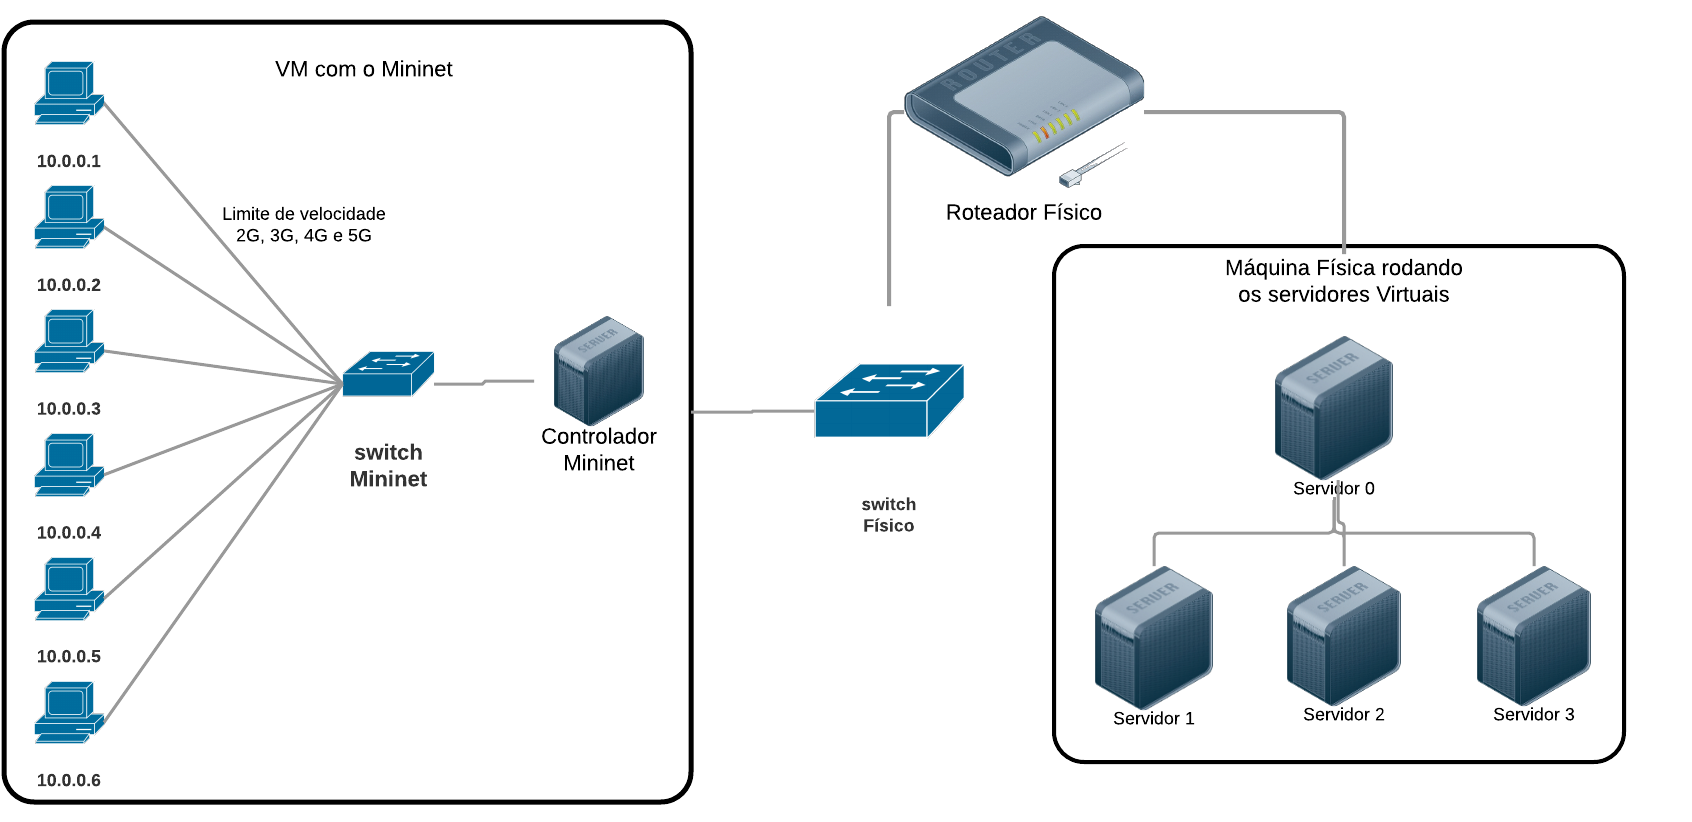
\includegraphics[width=1.0\columnwidth]{images/AmbienteTeste.png}
	\caption{Coniguração do ambiente utilizado para a realização dos experimentos. Fonte: Criada pelo autor.}
	\label{fig:cenarioConsiderado}
\end{figure}

Foi criado um script em Python, conforme Código \ref{src:python} com intuito de automatizar a criação dos hosts, limitar largura de banda entre 2G, 3G, 4G e 5G, iníciar a execução da aplicação responsável por simular as funcionalidades dos OBUs e RSUs,  realizar a comunicação com a arquitetura I9Vanet e registrar em log, os dados referentes à comunicação de cada host, em arquivos individuais.

Um host virtual tem a função de representar um veículo real, inclusive com uso de movimentações reais, coletadas por 12 meses, de um sistema de monitoramento de veículos de uma empresa de taxi com 102 carros, totalizando mais de 12 milhões de movimentações. A figura \ref{fig:monitoramento} mostra o exemplo do monitoramento do sistema de taxi.

\begin{figure}[t!]
	\centering
	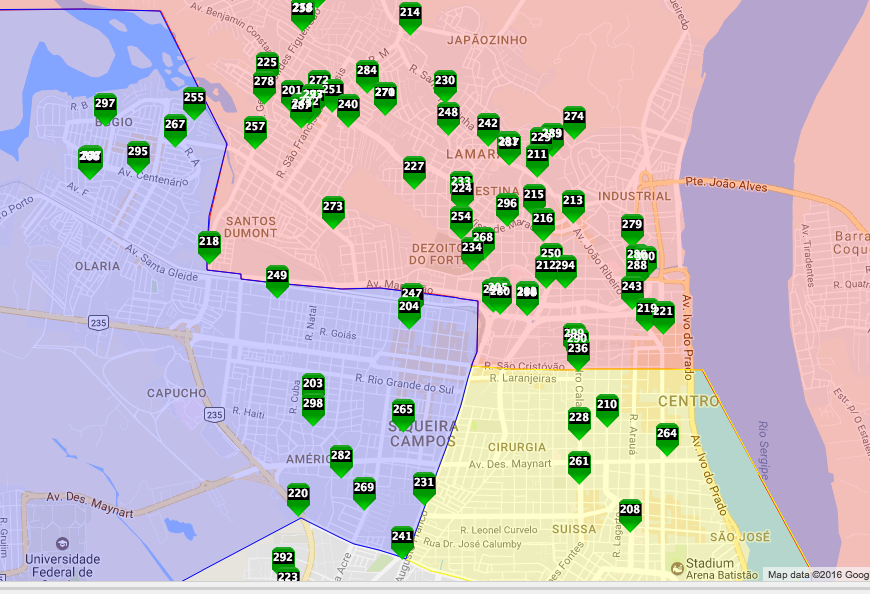
\includegraphics[width=1.0\columnwidth]{images/taxi_mapa.png}
	\caption{Tela de monitoramento do Sistema TaxiFast.}
	\label{fig:monitoramento}
\end{figure}


A base de movimentação foi extraída, separada por veículo e em seguida, armazenada em arquivo e colocada em cada máquina Mininet para que cada host pudesse simular uma  movimentação real. Cada arquivo de movimentação recebeu um número, por exemplo: 1.csv, 2.csv e assim por diante. Assim, os host virtuais realizaram um sorteio entre os arquivos disponíveis para ler as informações de movimentação e transmití-la para o servidor. A tabela \ref{tab:linhasArquivoMovimentacao} mostra exemplo do conteúdo de um arquivo de movimentação.


\begin{longtable}{ p{.30\textwidth}  p{.30\textwidth}   p{.30\textwidth}  p{.20\textwidth}} 
	\hline
	\rowcolor[gray]{0.7}
	Latitude	& Longitude	& Velocidade \\ \hline
	-10.9062183	& -37.0619264& 0 \\ \hline
	-10.906164143173685 & -37.061813870099655 & 10.7	\\ \hline	
	-10.904381347197752 & -37.0671766923126 & 21.121 \\ \hline
	-10.904279005332516  & -37.067784265675165 & 26.259 \\ \hline
	-10.904165425504841 & -37.06846398328098 & 29.678 \\ \hline
	\caption{Linhas do arquivo de movimentação.} 
	\label{tab:linhasArquivoMovimentacao}
\end{longtable}
\newpage
\begin{lstlisting}[caption=Script Python para criação dos hosts no mininet., label=src:python]
#!/usr/bin/python
...
class SingleSwitchTopo(Topo):
def build(self, n=2):
    switch = self.addSwitch('s1')
    #Cria todos os hosts e conecta ao switch
    for h in range(n):	
		host = self.addHost('h%s' % (h + 1))
		self.addLink(host, switch)
def limit( bw=0.2, cpu=1 ):
	intf = custom( TCIntf, bw=bw )
	myTopo = SingleSwitchTopo(n=2)
	for sched in 'rt', 'cfs':
	if sched == 'rt':
	release = quietRun( 'uname -r' ).strip('\r\n')
	output = quietRun( 'grep CONFIG_RT_GROUP_SCHED /boot/config-%s'
	% release )
	if output == '# CONFIG_RT_GROUP_SCHED is not set\n':
		continue
	host = custom( CPULimitedHost, sched=sched, cpu=cpu )
	net = Mininet( topo=myTopo, intf=intf, host=host)
	net.addNAT().configDefault()
	net.start()
	# Para cada host criado, executa a aplicacao de simulacao
	for host in net.hosts:
		if 'h' in host.name:
		   host.cmd('java -jar SVVMainTest.jar ' + str(host) + '.csv /home/mininet/vanet &')
	CLI( net )
if __name__ == '__main__':
setLogLevel( 'info' )
limit()
\end{lstlisting}

\section{Experimentos}

Ao iniciar cada teste do exprimento, os host virtuais devem estabelecer a conexão com o servidor nível 0, contudo, se todos os "veículos" iniciarem a conexão ao "mesmo tempo" ocasionará uma sobrecarga tanto na máquina cliente quanto no servidor. Pensando nisso, foi implementando na aplicação cliente que antes de iniciar o processo de conexão, cada host obtém um número pseudo-randômico entre 0 e 120000 (2 minutos), o qual será usado para dar uma pausa na aplicação pra depois iniciar o processo de conexão gerando assim, uma aleatoriedade inicial. Se por algum motivo a conexão do host cliente cair ou der \textit{timeout}, ela será refeita automaticamente não considerando mais o tempo de pausa inicial. 

******* Quais operações são realizadas a cada transmissão ver fluxo
******* Informar as velocidades de cada teste 2g, 3g ,4g, 5hg
% feito ******* explicar o sleep inicial de no máximo 2 min para inicia as requisições
% feito ******* colocar qnt hosts virtuais no mininet cada maquina fisica rodou
% feito ****** o servidor nível 0 chegou a 100\% de processamento nos primeiros 2 minutos no teste com 800 veículos  depois reduziu para 0.20 e se manteve, isso se deu devido à todas as conexoes iniciais serem feitas para este servidor, como também quando há a necessidade de mudança de domínio, o servidor nível 0 é requisitado de acordo com a hierarquia estabelecida.

% feito ****** para um melhor ganho de performançe é aconselhado que os domínios próximos fiquem no mesmo nível hierarquico um do outro à medida do possível, assim, o servidor pai, de nível mais acima irá encontrar mais rapidamente o servidor de destino, não precisando subir até o nível mais alto da árvore.
% feito ****** explicar que o cliente refaz a conexão caso perca, conectando-se ao ultimo servidor conectado
****** Por último foi executado o teste de stress sem o limite de banda - 800/10s=>80/s => 0,08s tempo médio de requisição, na prática o tempo ficou em 0,02s
%****** mostrar a mesma análise de execução porem  sem limite de banda 50,100,200,400,800,1600,3200

As máquinas utilizadas no experimento pertenciam a um laboratórios do Instituto Federal de Sergipe - Campus Lagarto e dois notebooks pertencente ao autor, cuja configurações estão presentes na tabela \ref{tab:configuracaoMaquinas}.

%Os experimentos foram divididos em 24 partes, levando em consideração a quantidade de hosts clientes, sendo 6 , e a velocidade na cumunicação, 

\begin{longtable}{ |p{.30\textwidth} |p{.10\textwidth}  |p{.45\textwidth}   |p{.10\textwidth} | p{.20\textwidth}} 
	\hline
	\rowcolor[gray]{0.7}
	 Maquina Cliente &	& 	&  \\ \hline
	\rowcolor[gray]{0.7}
	Sist Operacional.	& Qnt. & Processador	& Memória \\ \
	Windows 7	& 12 & AMD Phenom II X2 B57 3.20 GHz & 4 GB	\\ \
	Mac OS Sierra	& 1 & 2,4 GHz Intel Core i5	& 8 GB \\   \hline
	\rowcolor[gray]{0.7}
	 Maquina Servidora &	& 	&  \\ \hline
	\rowcolor[gray]{0.7}
	 Sist Operacional. &	& Processador	& Memória \\ \
	Ubuntu 16.4	& 1 & 2,4 GHz Intel Core i7 GHz & 8 GB	\\ \hline
	\caption{Configuração dos computadores utilizados no experimento. } 
	\label{tab:configuracaoMaquinas}
\end{longtable}

Para cada cenário, 50,100,200 e 400 veículos, os \textit{hosts} emulados seguiram a seguinte distribuição entre as máquinas clientes como mostra a tabela \ref{tab:configuracaoCenarios}, tendo como preocupação o poder de processamento das máquinas físicas.
%\begin{longtable}{ |p{.30\textwidth} |p{.10\textwidth}  |p{.45\textwidth} |} 
\begin{longtable}{ |c |c |c |} 
	\hline
	\rowcolor[gray]{0.7}
	Cenário 50 &	& 	  \\ \hline
	\rowcolor[gray]{0.7}
	Máquian Física.	& Qnt. & Nr \textit{Hosts} Cada	 \\ \hline
	Windows	& 2 & 25 	\\ \hline
	\rowcolor[gray]{0.7}
	Cenário 100 &	& 	  \\ \hline
	\rowcolor[gray]{0.7}
	Máquina Física.	& Qnt. & Nr \textit{Hosts} Cada	 \\ \hline
	Windows	& 4 & 25 	\\ \hline
	\rowcolor[gray]{0.7}	
	Cenário 200 &	& 	  \\ \hline
	\rowcolor[gray]{0.7}
	Máquina Física.	& Qnt. & Nr \textit{Hosts} Cada	 \\ \hline
	Windows	& 6 & 25 	\\ \hline
	Mac OS	& 1 & 50 	\\ \hline
	\rowcolor[gray]{0.7}	
	Cenário 400 &	& 	  \\ \hline
	\rowcolor[gray]{0.7}
	Máquina Física.	& Qnt. & Nr \textit{Hosts} Cada	 \\ \hline
	Windows	& 12 & 25 	\\ \hline
	Mac OS	& 2 & 50 	\\ \hline
	\caption{Configuração dos computadores utilizados no experimento em cada cenário. } 
	\label{tab:configuracaoCenarios}
\end{longtable}

Conforme dito anteriormente, foram definidos 48 cenários de testes levando em consideração quantidades de veículos, largura de banda da comunicação e a criptografia ou não dos dados.
%\begin{longtable}{ p{.20\textwidth}  p{.20\textwidth}   p{.20\textwidth}  p{.20\textwidth}} 
%	\hline
%	Quantidade Hosts	& Comunicação 2G	& Comunicação G3 & Comunicação 4G \\ \hline
%	10	& & &	\\ \
%	50	& & &	\\ \	\\ \hline
%	\caption{Colunas das tabelas da base de dados. Fonte: Criada pelo autor} % needs to go inside longtable environment
%	\label{tab:configuracaoQntVelocidade}
%\end{longtable}


\section{Resultados}

Inicialmente, os dados colhidos referentes à latência, foram avaliados quanto à sua normalidade, para verificar se a distribuição de probabilidade associada às amostras podem ser aproximada. Para tal, foi utilizado o Kolmogorov-Smirnov test (KS) tendo as seguintes hipóteses:

H0: Os dados seguem uma distribuição normal.

Ha: Os dados não seguem uma distribuição normal.

O resultado do teste KS aplicado às médias dos tempos de latência das requisições de cada \textit{host}, indica que nenhuma das amostras apresentou uma distribuição normal a um nível de significância, comumente utilizado, de 0,05, rejeitando a hipótese H0, como mostrado na Tabela \ref{tbEstatisticaKS}, apontando que a distribuição de probabilidade associada às médias das requisições não podem ser aproximadas.

\begin{table}[!h]
	\centering
	\caption{Resultado do teste de análise de distribuição normal dos dados para cada quantidade de veículos e velocidades de acesso. }
	\label{tbEstatisticaKS}
	\begin{tabular}{|p{4.0cm}|p{2.0cm}|p{2.0cm}|p{2.0cm}|p{2.0cm}|}
		\hline
		\rowcolor[gray]{0.7}
		Qnt. Veículos & 2G  & 3G  & 4G  & 5G  \\ \hline
		\cellcolor[gray]{0.7}50              & 0,0 & 0,0 & 0,0 & 0,0 \\ \hline
		\cellcolor[gray]{0.7}100             & 0,0 & 0,0 & 0,0 & 0,0 \\ \hline
		\cellcolor[gray]{0.7}200             & 0,0 & 0,0 & 0,0 & 0,0 \\ \hline
		\cellcolor[gray]{0.7}400             & 0,0 & 0,0 & 0,0 & 0,0 \\ \hline
		\cellcolor[gray]{0.7}800             & 0,0 & 0,0 & 0,0 & 0,0 \\ \hline
		\cellcolor[gray]{0.7}1600            & 0,0 & 0,0 & 0,0 & 0,0 \\ \hline
	\end{tabular}
\end{table}

Sob a ótica das variações entre as latências das requisições, podemos observar que nos cenários com 50 e 100 veículos, o coeficiente de variação foi baixa e acima de 200 veículos houve um crecimento no coeficiente. Isso aconteceu devido à maior quantidade de veículos presente nos testes e consequentemente, houve mais mudança de servidores, em média o tempo gasto para realizar a operação \textit{changeServer} é de 2,5 segundos, conforme mostra a tabela \ref{tbEstatisticaVariacoes}.

\begin{table}[!h]
	\centering
	\caption{Resultado do teste de análise dos coeficientes de variação.}
	\label{tbEstatisticaVariacoes}
	\begin{tabular}{|p{4.0cm}|p{2.0cm}|p{2.0cm}|p{2.0cm}|p{2.0cm}|}
		\hline
		\rowcolor[gray]{0.7}
		Qnt. Veículos & 2G      & 3G     & 4G     & 5G      \\ \hline
		\cellcolor[gray]{0.7}50              & 0.52360 & 0.5504 & 0.5751 & 0.5435 \\ \hline
		\cellcolor[gray]{0.7}100             & 0.5340  & 0.5490 & 0.5630 & 0.5560  \\ \hline
		\cellcolor[gray]{0.7}200             & 2.1970  & 2.5930 & 2.4360 & 2.3560  \\ \hline
		\cellcolor[gray]{0.7}400             & 1.9220  & 2.1680 & 2.4270 & 2.5360  \\ \hline
	\end{tabular}
\end{table}

As imagens contidas na figura \ref{fig:imgHistFreq50}, mostram o histógrama de frequência das médias das requisições para cada velocidade, 2G, 3G, 4G e 5G, para o teste com 50 veículos. Observou-se que não há uma relação de melhora nos tempos médios à medida que aumenta a velocidade de 2G para 5G.  A concentração dos tempos permanecem na mesma referência, entre 40 e 50 milisegundos.

\begin{figure}[ht]
	\caption{Análise de Histograma de Frequência do Teste  com 50 veículos.}
	\centering
	\label{fig:imgHistFreq50}
	\subfloat[ 2G]{
		%width=0.5\linewidth
		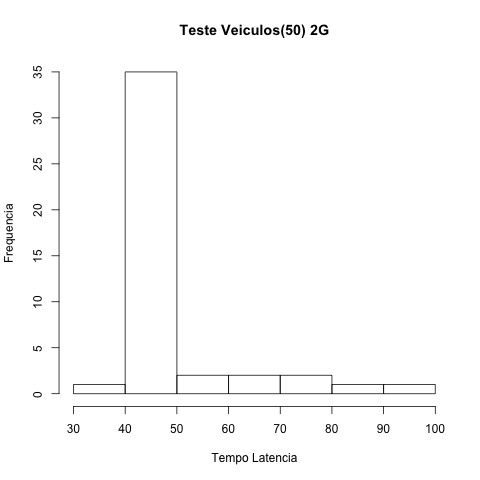
\includegraphics[width=5cm,height=5cm]{images/hist_media2g50.jpg}
		\label{fig:imgGraficoFreq2g50}
	}
	\subfloat[3G]{
		%width=0.5\linewidth
		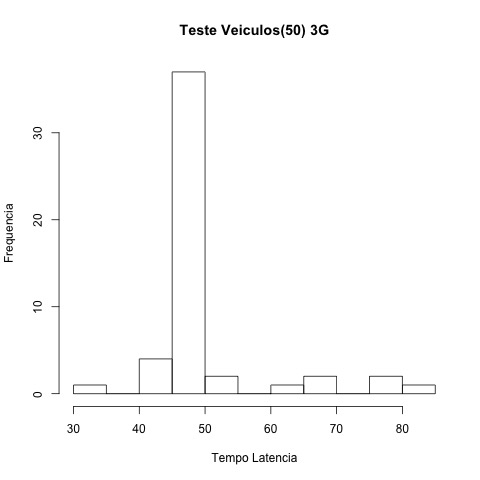
\includegraphics[width=5cm,height=5cm]{images/hist_media3g50.jpg}
		\label{fig:imgGraficoFreq3g50}
	}
	\\
	\subfloat[w4G]{
		%width=0.5\linewidth
		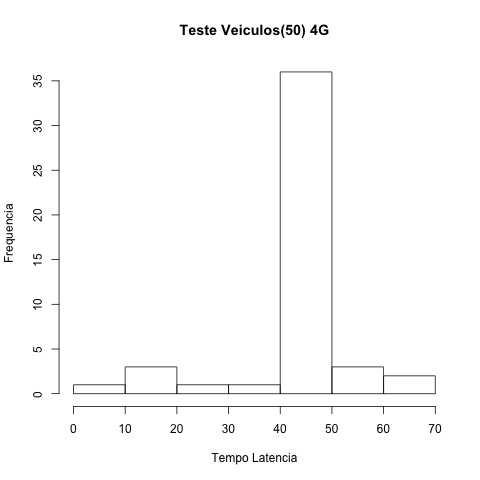
\includegraphics[width=5cm,height=5cm]{images/hist_media4g50.jpg}
		\label{fig:imgGraficoFreq4g50}
	}	
	\subfloat[5G]{
		%width=0.5\linewidth
		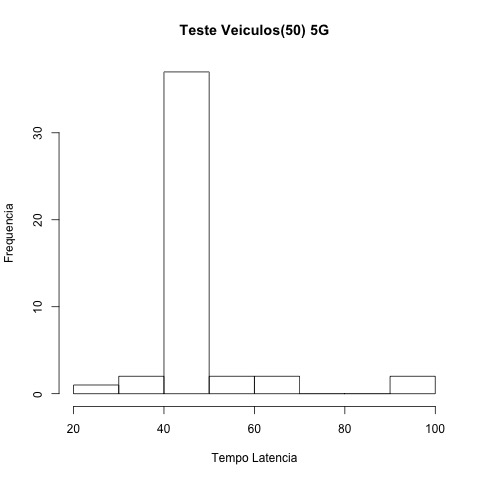
\includegraphics[width=5cm,height=5cm]{images/hist_media5g50.jpg}
		\label{fig:imgGraficoFreq5g50}
	}
\end{figure}


O cenário com 100 veículos apresentou gráficos semalhantes aos de 50, ou seja, o tempo médio das requisições não variou de acordo com o aumento da velocidade, conforme mostra a figura \ref{fig:imgHistFreq100}.

\begin{figure}[ht]
	\caption{Análise de Histograma de Frequência do Teste  com 100 veículos.}
	\centering
	\label{fig:imgHistFreq100}
	\subfloat[ 2G]{
		%width=0.5\linewidth
		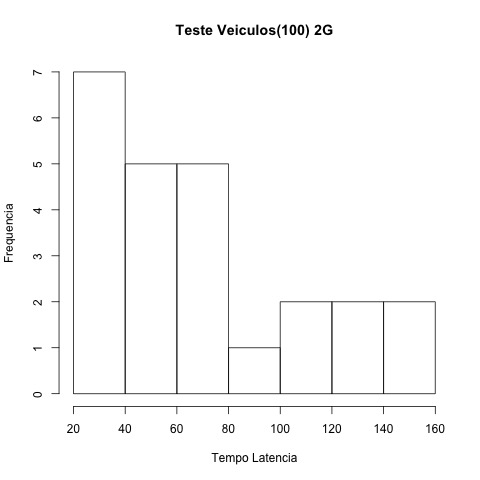
\includegraphics[width=5cm,height=5cm]{images/hist_media2g100.jpg}
		\label{fig:imgGraficoFreq2g100}
	}
	\subfloat[3G]{
		%width=0.5\linewidth
		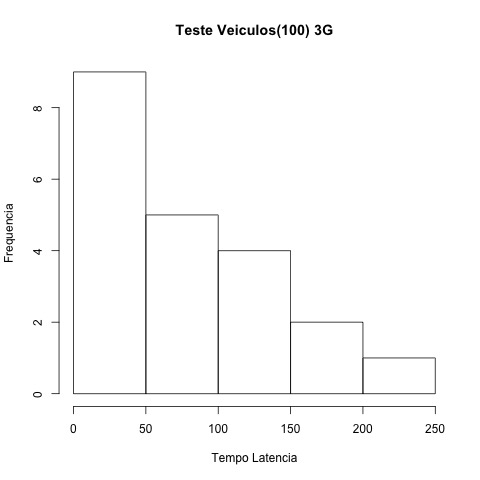
\includegraphics[width=5cm,height=5cm]{images/hist_media3g100.jpg}
		\label{fig:imgGraficoFreq3g100}
	}
	\\
	\subfloat[4G]{
		%width=0.5\linewidth
		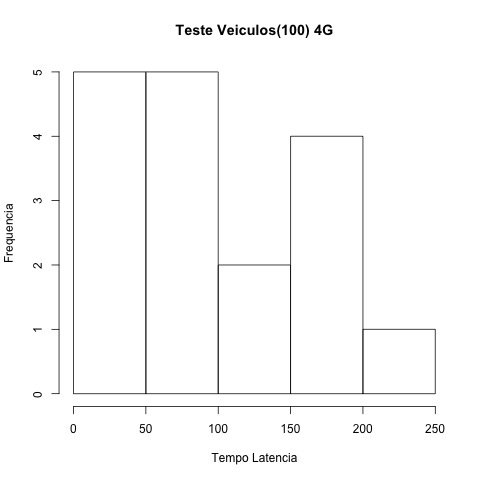
\includegraphics[width=5cm,height=5cm]{images/hist_media4g100.jpg}
		\label{fig:imgGraficoFreq4g1000}
	}	
	\subfloat[5G]{
		%width=0.5\linewidth
		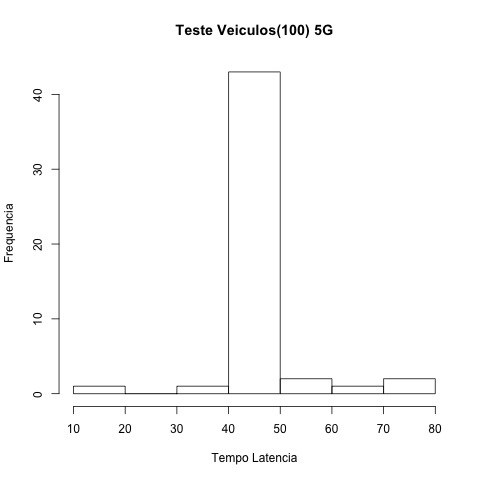
\includegraphics[width=5cm,height=5cm]{images/hist_media5g100.jpg}
		\label{fig:imgGraficoFreq5g100}
	}
\end{figure}

Entretanto, os testes com o cenário de 200 veículos, apresentou uma variação com a diferença de velocidades porém, de maneira inversamente proporcional, ou seja, de acordo com a figura \ref{fig:imgHistFreq200}, o teste com a velocidade 2G apresentou maior concentração entre o intervalo de 0 e 50 milisegundos. Com a velocidade de 3G a maior concentração dos tempos médios ficou entre 140 e 160 milisegundos.
 
\begin{figure}[ht]
	\caption{Análise de Histograma de Frequência do Teste  com 200 veículos.}
	\centering
	\label{fig:imgHistFreq200}
	\subfloat[ 2G]{
		%width=0.5\linewidth
		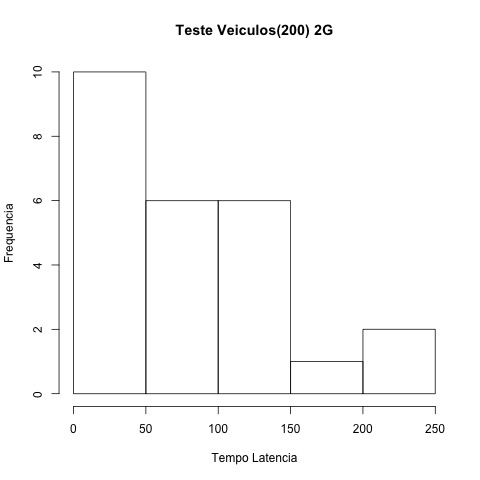
\includegraphics[width=5cm,height=5cm]{images/hist_media2g200.jpg}
		\label{fig:imgGraficoFreq2g200}
	}
	\subfloat[3G]{
		%width=0.5\linewidth
		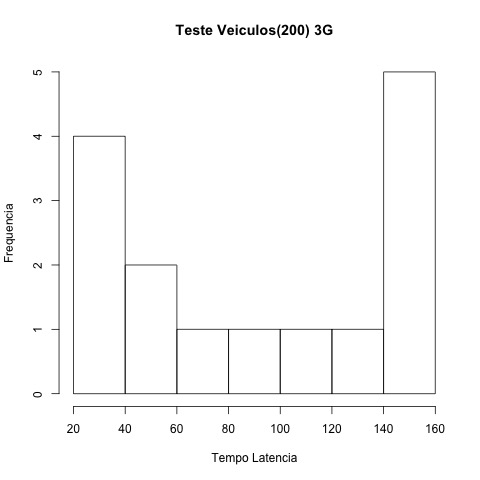
\includegraphics[width=5cm,height=5cm]{images/hist_media3g200.jpg}
		\label{fig:imgGraficoFreq3g200}
	}
	\\
	\subfloat[4G]{
		%width=0.5\linewidth
		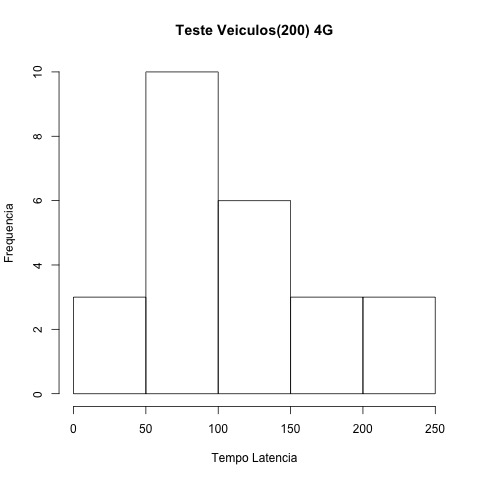
\includegraphics[width=5cm,height=5cm]{images/hist_media4g200.jpg}
		\label{fig:imgGraficoFreq4g200}
	}	
	\subfloat[5G]{
		%width=0.5\linewidth
		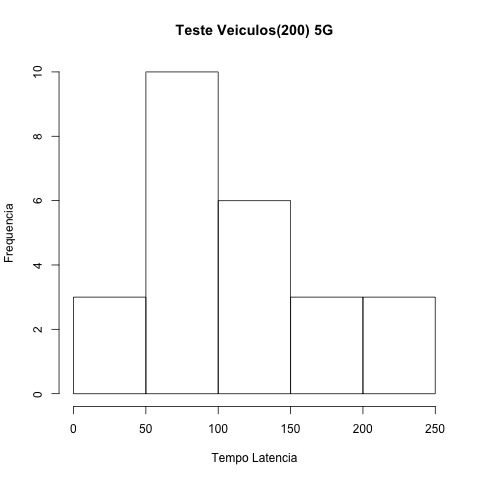
\includegraphics[width=5cm,height=5cm]{images/hist_media5g200.jpg}
		\label{fig:imgGraficoFreq5g200}
	}
\end{figure}

Da mesma maneira que o cenário com 200 veículos, o de 400 não apresentou uma relação lógica sendo que a velocidade 2G mostrou, de forma considerável, médias entre 600 e 700 milisegundos  como mostra a figura \ref{fig:imgHistFreq400}.

\begin{figure}[ht]
	\caption{Análise de Histograma de Frequência do Teste  com 400 veículos.}
	\centering
	\label{fig:imgHistFreq400}
	\subfloat[ 2G]{
		%width=0.5\linewidth
		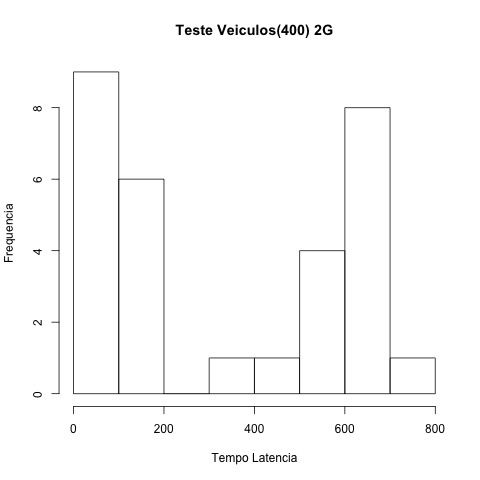
\includegraphics[width=5cm,height=5cm]{images/hist_media2g400.jpg}
		\label{fig:imgGraficoFreq2g40}
	}
	\subfloat[3G]{
		%width=0.5\linewidth
		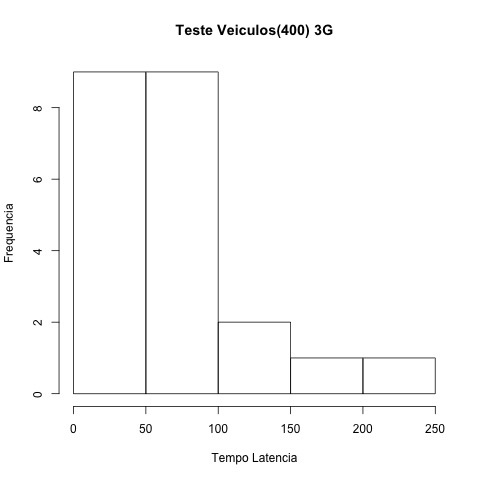
\includegraphics[width=5cm,height=5cm]{images/hist_media3g400.jpg}
		\label{fig:imgGraficoFreq3g400}
	}
	\\
	\subfloat[4G]{
		%width=0.5\linewidth
		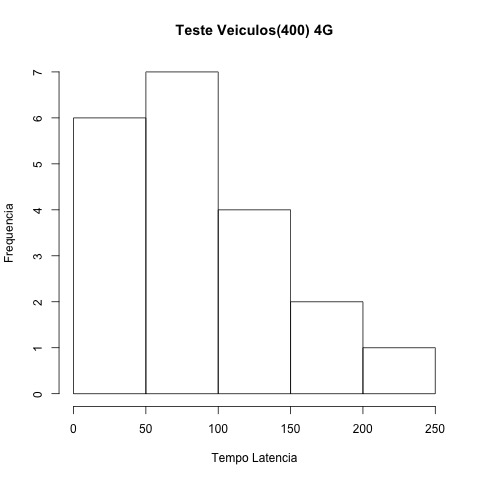
\includegraphics[width=5cm,height=5cm]{images/hist_media4g400.jpg}
		\label{fig:imgGraficoFreq4g400}
	}	
	\subfloat[5G]{
		%width=0.5\linewidth
		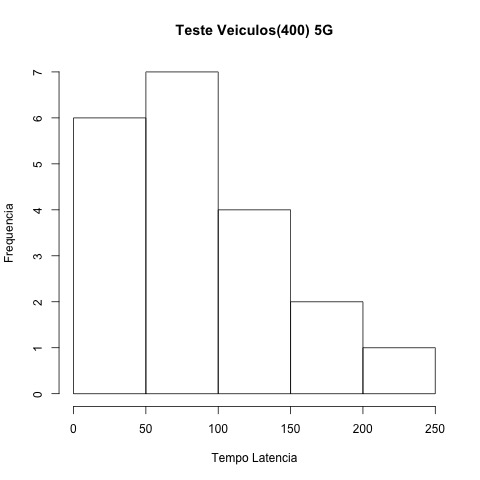
\includegraphics[width=5cm,height=5cm]{images/hist_media5g400.jpg}
		\label{fig:imgGraficoFreq5g400}
	}
\end{figure}



%%%%%%%%%  Tabelas Comparativo Tempos Min, Médio e Máximos entre os cenários
%\begin{table}[!h]
%	\centering
%	\caption{Tempos mínimos, máximos e a média para 2G e 3G.}
%	\label{tbEstatisticaMMM}
%\begin{tabular}{|c|r|r|r|r|r|r|r|r|r|}
%	\hline
%	\rowcolor[gray]{0.7}
%	 &  \multicolumn{3}{| c| }{2G} & \multicolumn{3}{ |c| }{3G}  \\ \hline
%	\rowcolor[gray]{0.7}
%	 Qnt. Veciulos & Min & Média & Max & Min & Média & Max   \\ \hline
%	\cellcolor[gray]{0.7}50 & 30,50 & 51,12 & 91,50 & 32,74 & 50,540 & 81,00   \\ \hline
%	\cellcolor[gray]{0.7}100 & 30,92, & 68,83 & 143,40 & 31,19 & 82.89 & 210,00   \\ \hline
%	\cellcolor[gray]{0.7}200 & 31,35  & 86,13 & 241,90 & 29,56 & 92,09 & 155,10   \\ \hline
%	\cellcolor[gray]{0.7}400 & 33,93 & 337,20 & 713,50 & 37,87 & 79,16 & 238,50   \\ \hline
%\end{tabular}
%\end{table}

%\begin{table}[!h]
%	\centering
%	\caption{Tempos mínimos, máximos e a média para 4G e 5G.}
%	\label{tbEstatisticaMMM}
%	\begin{tabular}{|c|r|r|r|r|r|r|r|r|r|}
%		\hline
%		\rowcolor[gray]{0.7}
%		&  \multicolumn{3}{| c| }{4G} & \multicolumn{3}{ |c| }{5G}  \\ \hline
%		\rowcolor[gray]{0.7}
%		Qnt. Veciulos & Min & Média & Max & Min & Média & Max   \\ \hline
%		\cellcolor[gray]{0.7}50 & 32,50 & 45,33 & 68,96 & 29,31 & 49,44  & 91,50   \\ \hline
%		\cellcolor[gray]{0.7}100 & 34,83 & 99,94 & 242,60 & 18,50 & 48,35  & 78,53   \\ \hline
%		\cellcolor[gray]{0.7}200 & 37,13 & 108,50 & 249,40 & 37,13 & 109,13 & 249,40   \\ \hline
%		\cellcolor[gray]{0.7}400 & 46,33 & 92,69 & 217,80  & 46,33 & 92,69 & 217,80  \\ \hline
%	\end{tabular}
%\end{table}

Nas figuras \ref{fig:graficotempomin},  \ref{fig:graficotempomedio} e  \ref{fig:graficotempomax}, é feito uma análise sobre os tempos mínimos, médios e máximos das médias das latências das requisições extraídas de casa cenário. Fica evidente que nos cenários de 50, 100 e 200 veículos simultâneos, os tempos mínimos, médios e máximos sofrem pequena variação porém, os tempos médios e máximos no cenário com 400 veículos com velocidade de 2G, há um aumento considerável em relação às outras velocidades, como mostra as figuras \ref{fig:graficotempomedio} e  \ref{fig:graficotempomax}.

\begin{figure}[t!]
	\centering
	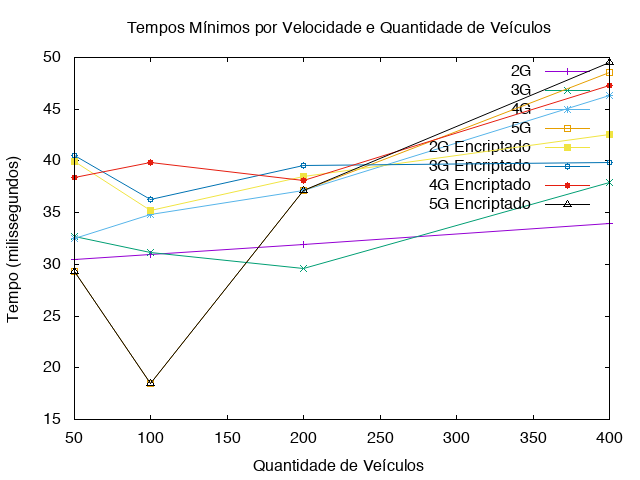
\includegraphics[width=0.7\columnwidth]{images/grafico_tempo_min.png}
	\caption{Gráfico comparativo dos tempos mínimos entres os cenários.}
	\label{fig:graficotempomin}
\end{figure}

\begin{figure}[t!]
	\centering
	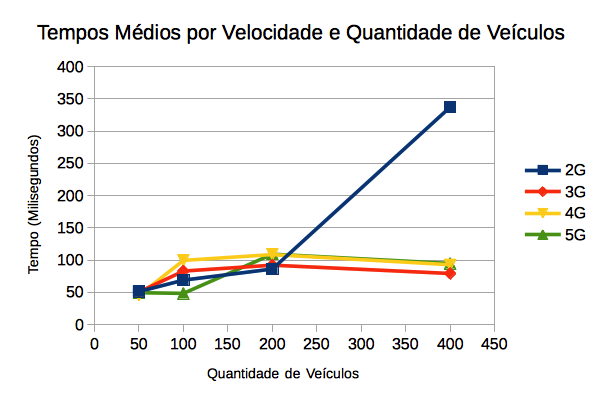
\includegraphics[width=0.7\columnwidth]{images/grafico_tempo_medio.png}
	\caption{Gráfico comparativo dos tempos médios entres os cenários.}
	\label{fig:graficotempomedio}
\end{figure}

\begin{figure}[t!]
	\centering
	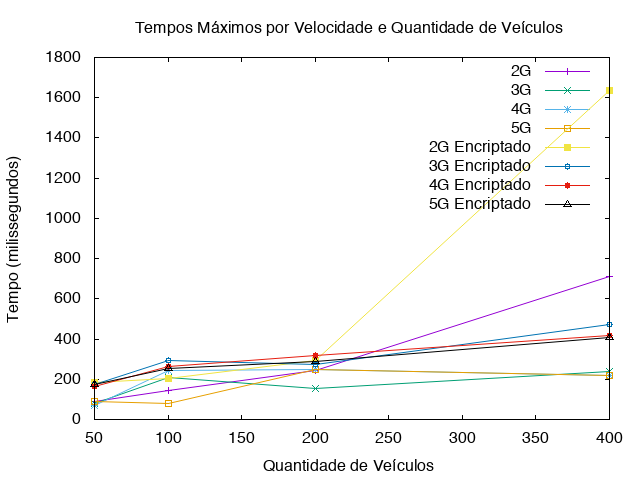
\includegraphics[width=0.7\columnwidth]{images/grafico_tempo_max.png}
	\caption{Gráfico comparativo dos tempos máximos entres os cenários.}
	\label{fig:graficotempomax}
\end{figure}

\subsection{Taxa de Transferência}

Os veículo enviam sua localização, através do comando \textit{sendMoviment}, a cada 10 segundos sendo que a mensagem enviada variou entre 212 e 256 bytes e a média ficou em 233 bytes então, a tabela \ref{tbLink} mostra as velocidades de transmissão utilizadas em cada teste e a capacidade de operação de cada link testado. 

\begin{table}[!h]
	\centering
	\caption{Velocidade de cada link por veículo.}
	\label{tbLink}
	\begin{tabular}{|p{2.0cm}|p{4.0cm}|p{3.0cm}|p{2.0cm}|p{2.0cm}|}
		\hline
		\rowcolor[gray]{0.7}
		Link & Lagura de Banda(kbps)           \\ \hline
		\cellcolor[gray]{0.7}2G              & 400  \\ \hline
		\cellcolor[gray]{0.7}3G             & 10.000    \\ \hline
		\cellcolor[gray]{0.7}4G             & 100.000    \\ \hline
		\cellcolor[gray]{0.7}5G             & 10.000.000    \\ \hline
	\end{tabular}
\end{table}


\subsection{Processamento}

Também foi avaliado o nível de processamento dos servidores, sendo que o servidor nível 0 chegou a 100\% de processamento nos primeiros 2 minutos, no teste com 800 veículos, e depois reduziu para 20\%, onde se manteve. Isso ocorreu devido à todas as conexoes iniciais serem feitas para este servidor, como também quando há a necessidade de mudança de domínio, o servidor nível 0 é requisitado de acordo com a hierarquia estabelecida. 

\chapter{Conclusão e Trabalhos Futuros}\label{sec:conclusao}

\section{Conclusões deste Trabalho}
O presente trabalho apresentou o modelo de uma arquitetura para rede veiculares em nuvem, denominado i9Vanets, como também uma avaliação com intuito de medir a sua eficácia e eficiência, visando atender às demandas e desafios relacionados à VANETs. Este modelo permite montar uma rede veicular em nuvem e realizar todo gerenciamento e comunicação de maneira virtual, tornando os equipamentos OBUs e RSUs mais simples e baratos.

Foram realizados alguns testes estatísticos, com objetivo de analisar o comportamento da arquitetura. Sobre o teste da normalidade da distribuição, tanto no cliente quanto no servidor, foi constatado que distribuição de probabilidade associada às amostras não podem ser aproximada. Outra análise foi relacionado à dispersão dos dados através do coeficiente de variação, o qual avaliou, sobre as amostras de latência, que a dispersão em cada teste define um comportamento semelhante, porém, o coeficiente de variação medido em cima do tempo de processamento no servidor, mostrou que os testes 250, 500, 1000, 2000 e 2500 tiveram grande dispersão.

Em relação ao nível de processamento dos servidores, o servidor nível 0 é o responsável pelas primeiras conexões feitas pelos veículos e durante a mudança de domínios, pensando nisso, para uma melhor organização e diminuição de carga em um único servidor, é interessante que os domínios vizinhos fiquem, ao máximo, no mesmo nível de hierarquia tendo o mesmo servidor pai, assim, essa sub-árvore responderia de maneira mais eficiente ao comando \textit{changeServer} e diminuindo a pressão sobre o servidor nível raiz.

Uma outra possibilidade é que o serividor nível 0 seja utilizado apenas para coordenar a estrutura retirando de si o papel de gerenciar os veículos, assim ele teria o papel de receber as primeiras conexões dos veículos e encaminhá-las para o servidor correspondente, o mesmo na operação \textit{changeServer}'.

* a velocidade 2G e 5G apresentam os mesmos tempos médios


\section{Trabalhos Futuros}

Como trabalhos futuros, é possível criar várias aplicações tais como: sistema de detecção e alerta de congestionamento de trânsito, permitindo um RSU avisar a outros RSU e/ou OBU; Controle de passagem livre para veículos de urgência e emergência; utilizar a arquitetura pra criar um simulador que possa simular toda uma cidade; Criar novos algoritmos de roteamento, segurança e comunicação.
% ----------------------------------------------------------
% ELEMENTOS PÓS-TEXTUAIS
% ----------------------------------------------------------
\postextual
% ----------------------------------------------------------

% ----------------------------------------------------------
% Referências bibliográficas
% ----------------------------------------------------------
\bibliography{referencias}

% ----------------------------------------------------------
% Glossário
% ----------------------------------------------------------
%
% Consulte o manual da classe abntex2 para orientações sobre o glossário.
%
%\glossary

% ----------------------------------------------------------
% Apêndices
% ----------------------------------------------------------

% ---
% Inicia os apêndices
% ---
%\begin{apendicesenv}
%\end{apendicesenv}
% ---


% ----------------------------------------------------------
% Anexos
% ----------------------------------------------------------

% ---
% Inicia os anexos
% ---
%\begin{anexosenv}
%\end{anexosenv}

%---------------------------------------------------------------------
% INDICE REMISSIVO
%---------------------------------------------------------------------
%%%%%MF\phantompart
%%%%%MF\printindex
%---------------------------------------------------------------------

\end{document}
